% ============================================================
%  Práctica Experimental N.° 4 -- Unidad IV
%  Validación, Gestión de Requisitos y Herramientas CASE
%  Asignatura: Ingeniería de Requerimientos [20303] -- UTEQ 2026-2027
%  Sistema del PFC: MundiPets
%  Formato: IEEE onecolumn | Biber + biblatex (estilo IEEE)
% ============================================================
\documentclass[journal,onecolumn]{IEEEtran}

% ── Codificación e idioma ───────────────────────────────────
\usepackage[T1]{fontenc}
\usepackage[utf8]{inputenc}
\usepackage[spanish, es-tabla]{babel}
\usepackage[autostyle=true, spanish=mexican]{csquotes}

% ── Tablas ──────────────────────────────────────────────────
\usepackage{booktabs}
\usepackage{tabularx}
\usepackage{array}
\usepackage{multirow}
\usepackage{longtable}
\newcolumntype{C}[1]{>{\centering\arraybackslash}p{#1}}
\newcolumntype{L}[1]{>{\raggedright\arraybackslash}p{#1}}

% ── Figuras ─────────────────────────────────────────────────
\usepackage{graphicx}
\usepackage{float}

% ── Color y enlaces ─────────────────────────────────────────
\usepackage{xcolor}

% ── Geometría ───────────────────────────────────────────────
\usepackage{geometry}
\geometry{a4paper, top=2.5cm, bottom=2.5cm, left=2.5cm, right=2.5cm, headheight=14pt, footskip=1.2cm}

% ── Encabezado ──────────────────────────────────────────────
\usepackage{fancyhdr}
\pagestyle{fancy}
\fancyhf{}
\renewcommand{\headrulewidth}{0.4pt}
\fancyhead[L]{\small Práctica Experimental 4 -- Ingeniería de Requerimientos}
\fancyhead[R]{\small MundiPets -- Validación y Gestión de Requisitos}
\fancyfoot[C]{\thepage}

% ── Espaciado y Parches ─────────────────────────────────────
\usepackage{parskip}
\setlength{\parskip}{4pt}
\makeatletter
\@ifundefined{labelindent}{}{\let\labelindent\relax}
\makeatother
\usepackage{enumitem}
\usepackage{caption}
\usepackage{titlesec}
\captionsetup{font=small, labelfont=bf}
\usepackage{amssymb}
\usepackage{amsmath}
\setlength{\emergencystretch}{2em}

% ── Forzar "Tabla" en lugar de "Cuadro" ──────────────────────
\renewcommand{\thetable}{\arabic{table}}
\def\tablename{Tabla}

% ── Formato de Secciones ────────────────────────────────────
\renewcommand{\thesection}{\arabic{section}}
\renewcommand{\thesubsection}{\thesection.\arabic{subsection}}
\renewcommand{\thesubsubsection}{\thesubsection.\arabic{subsubsection}}

\titleformat{\section}{\normalfont\Large\bfseries}{\thesection}{1em}{}
\titleformat{\subsection}{\normalfont\large\bfseries}{\thesubsection}{1em}{}
\titleformat{\subsubsection}{\normalfont\normalsize\bfseries}{\thesubsubsection}{1em}{}

% ── Bibliografía: biblatex + biber, estilo IEEE ──────────────
\usepackage[
backend=biber,
style=ieee,
citestyle=numeric-comp,
isbn=true,
doi=true
]{biblatex}
\addbibresource{referencias.bib}

\usepackage[hidelinks,colorlinks=false]{hyperref}

\setcounter{secnumdepth}{4}
\setcounter{tocdepth}{4}

\begin{document}
	
	% ═══════════════════════════════════════════════════════════════
	%  CARÁTULA
	% ═══════════════════════════════════════════════════════════════
	\begin{titlepage}
		\centering
		
		{\large\bfseries UNIVERSIDAD TÉCNICA ESTATAL DE QUEVEDO\\[12pt]}
		
		
\includegraphics[width=0.3\textwidth]{figuras/logo_uteq.png}\\[12pt]
		
		{\large\bfseries FACULTAD DE CIENCIAS DE LA COMPUTACIÓN\\[4pt]
			CARRERA DE INGENIERÍA EN SOFTWARE}
		
		\vspace{0.8cm}
		
		{\normalsize\bfseries TEMA:}\\[4pt]
		{\normalsize PRÁCTICA EXPERIMENTAL 4 -- UNIDAD IV:\\
			VALIDACIÓN, GESTIÓN DE REQUISITOS Y HERRAMIENTAS CASE\\
			SISTEMA: MUNDIPETS}\\[4pt]
		
		\vspace{0.5cm}
		
		{\normalsize\bfseries MATERIA:}\\[4pt]
		{\normalsize INGENIERÍA DE REQUERIMIENTOS}
		
		\vspace{0.5cm}
		
		{\normalsize\bfseries DOCENTE:}\\[4pt]
		{\normalsize ING. GLEISTON CICERÓN GUERRERO ULLOA, PhD}
		
		\vspace{0.5cm}
		
		{\normalsize\bfseries INTEGRANTES Y ROLES:}\\[6pt]
		
		\textit{\textbf{FUERTES ARRAES EDSON DANIEL}},~CI: 0929115087,~Correo: efuertesa2@uteq.edu.ec\\
		\textit{Moderador de la inspección -- Presidente del CCB -- Integración y línea base}\\[6pt]
		
		\textit{CONTRERAS CHÁVEZ KEVIN GERMÁN},~CI: 1251167720,~Correo: kcontrerasc3@uteq.edu.ec\\
		\textit{Lector de la inspección -- Inspector 2 -- Analista del CCB}\\[6pt]
		
		\textit{VITERI GARCÍA JONATHAN ENRIQUE},~CI: 1250424734,~Correo: Jonathanvg2407@gmail.com\\
		\textit{Inspector 1 -- Representante del cliente en el CCB}
		
		\vspace{0.5cm}
		
		{\normalsize\bfseries CURSO:}\\[4pt]
		{\normalsize CUARTO SEMESTRE PARALELO ``B''}
		
		\vspace{0.5cm}
		
		{\normalsize\bfseries Versión del ERS resultante:} v1.1 \quad
		{\normalsize\bfseries Baseline:} \texttt{baseline-v1.1}
		
		\vspace{0.3cm}
		
		{\normalsize\bfseries REPOSITORIO:}\\
		\url{https://github.com/MiloSaurio4kHD/ISR401-PFC-ERS-EQUIPO-E}
		
		\vspace{0.8cm}
		
		{\normalsize\bfseries QUEVEDO -- LOS RÍOS -- ECUADOR}\\[4pt]
		{\normalsize\bfseries 2026 -- 2027 PPA}
		
	\end{titlepage}
	
	% ═══════════════════════════════════════════════════════════════
	%  SECCIÓN 1 -- RESUMEN Y OBJETIVOS
	% ═══════════════════════════════════════════════════════════════
	\section{Resumen y objetivos}
	
	\subsection{Resumen}
	
	\subsection{Objetivo general}
	
	\subsection{Objetivos específicos}
	
	% ═══════════════════════════════════════════════════════════════
	%  SECCIÓN 2 -- FUNDAMENTO TEÓRICO
	% ═══════════════════════════════════════════════════════════════
	\section{Fundamento teórico}
	
	\subsection{Marco normativo}
	
	La Ingeniería de Requisitos de MundiPets exige una especificación comprensible, verificable,
	validada y controlada durante toda su evolución. Para el contenido normativo de este apartado se
	utilizan las normas ISO/IEC/IEEE 29148:2018 \cite{iso29148} e ISO/IEC 25010 \cite{iso25010v2011,
		iso25010}, complementadas metodológicamente por SWEBOK v4.0 \cite{swebok4}, Pohl \cite{pohl2025}
	y el PMBOK 7.ª edición \cite{pmbok7}.
	
	\subsubsection{ISO/IEC/IEEE 29148:2018 y la validación de requisitos}
	
	La norma presenta un tratamiento unificado de los procesos y productos de la Ingeniería de
	Requisitos a lo largo del ciclo de vida. Ubica la definición de requisitos del sistema y del
	software en el apartado 6.4 y las actividades relacionadas con la validación en el 6.5.3. Además,
	define \emph{requirements validation} como la confirmación de que los requisitos describen el
	sistema correcto según la intención de los stakeholders, y \emph{requirements verification} como
	la confirmación de que los requisitos están bien formados \cite{iso29148}.
	
	Esta distinción es directamente aplicable a MundiPets. El ERS define RF-09 para la validación de
	información médica y, al mismo tiempo, en el conflicto ``Validación documental limitada''
	establece que debe emplearse ``validación referencial'' y no ``certificación clínica''. Por ello
	la inspección debe revisar tanto la forma del requisito como su coherencia con el alcance y con
	las expectativas registradas en la Entrega 2A.
	
	La misma norma define la gestión de requisitos como el conjunto de actividades destinadas a
	identificar, documentar, mantener, comunicar, trazar y seguir requisitos durante el ciclo de vida,
	y define la trazabilidad como la identificación y documentación del camino de derivación hacia
	arriba y de asignación hacia abajo \cite{iso29148}. Estas definiciones permiten justificar que una
	modificación no debe tratarse como un cambio aislado de texto, sino como una modificación con
	impacto sobre los artefactos enlazados. Los procesos de ciclo de vida que enmarcan ese control de
	cambios están descritos en ISO/IEC/IEEE 12207:2017 \cite{iso12207} para software y en
	ISO/IEC/IEEE 15288:2023 \cite{iso15288} para sistemas.
	
	En la PE4 este principio se materializa mediante solicitudes formales de cambio (RFC), análisis de
	impacto, decisión del Change Control Board y establecimiento de una nueva línea base. En
	MundiPets, por ejemplo, una modificación de privacidad en RF-25 obliga a revisar RF-11, RNF-16,
	RD-04, la matriz de trazabilidad y los casos de prueba asociados.
	
	\subsubsection{ISO/IEC 25010: modelo de calidad aplicado a los RNF}
	
	La edición de 2011 definía un modelo de calidad en uso con cinco características y un modelo de
	calidad del producto con ocho: adecuación funcional, eficiencia de desempeño, compatibilidad,
	usabilidad, fiabilidad, seguridad, mantenibilidad y portabilidad \cite{iso25010v2011}. La norma
	indica que estas características pueden utilizarse para especificar y evaluar requisitos de
	calidad, establecer criterios de aceptación y revisar la completitud de una especificación; la
	revisión de 2023 mantiene ese uso y reorganiza el modelo de producto \cite{iso25010}.
	
	Aplicado a MundiPets, el modelo sirve como lista de comprobación para los RNF de la Entrega 2A. Se
	observan requisitos vinculados con desempeño (RNF-03), usabilidad (RNF-04), fiabilidad y
	disponibilidad (RNF-02 y RNF-08), seguridad y confidencialidad (RNF-01, RNF-05 y RNF-16),
	mantenibilidad (RNF-10), portabilidad (RNF-11), compatibilidad e interoperabilidad (RNF-09) y
	adecuación funcional de los componentes inteligentes (RNF-06 y RNF-07). RNF-12 se conserva como
	condición de escalabilidad declarada por el propio ERS, sin forzar una equivalencia distinta de la
	terminología del documento fuente.
	
	\subsubsection{SWEBOK v4.0, Pohl y el control de cambios}
	
	SWEBOK v4.0 organiza la Ingeniería de Requisitos como un área que abarca elicitación, análisis,
	especificación, validación y gestión \cite{swebok4}. Pohl trata la validación y la gestión de
	requisitos como actividades continuas orientadas a descubrir defectos, resolver conflictos y
	mantener alineadas las necesidades de los stakeholders con una especificación que evoluciona
	\cite{pohl2025}. Para MundiPets esto implica revisar no solo requisitos individuales, sino también
	consistencia, completitud, verificabilidad y trazabilidad del conjunto.
	
	Esta perspectiva justifica la inspección formal de la Sección 3 del ERS, donde se concentran los
	25 RF, los 16 RNF y las 9 RD. La revisión debe detectar contradicciones entre requisitos, términos
	ambiguos, datos omitidos y enlaces de trazabilidad que conduzcan a casos de uso con una finalidad
	distinta.
	
	\subsubsection{Change Control Board (CCB)}
	
	El control integrado de cambios requiere registrar las solicitudes, analizar su impacto y tomar
	una decisión antes de alterar una línea base. En ese marco, el CCB actúa como instancia de
	evaluación y decisión sobre cambios relevantes, considerando alcance, costo, riesgo y artefactos
	afectados \cite{pmbok7}. En esta PE4, Kevin Contreras participa como Analista del CCB y presenta
	el impacto técnico de RFC-01 y RFC-03.
	
	En conjunto, ISO/IEC/IEEE 29148:2018 aporta los conceptos de verificación, validación, gestión y
	trazabilidad de requisitos; ISO/IEC 25010 aporta un marco de calidad para revisar los RNF; SWEBOK
	y Pohl complementan las prácticas de Ingeniería de Requisitos; y el CCB formaliza las decisiones
	que deben reflejarse en la versión resultante del ERS de MundiPets.
	
	\subsection{Validación de requisitos}
	
	\subsubsection{Verificación y validación}
	
	Verificación y validación responden preguntas distintas. La verificación de requisitos confirma
	que el enunciado o el conjunto de requisitos está bien formado y cumple las características
	esperadas de una buena especificación. La validación confirma que esos requisitos representan el
	sistema correcto para el uso previsto y las expectativas de los stakeholders \cite{iso29148}. En
	términos prácticos, la verificación pregunta si el requisito está redactado correctamente; la
	validación pregunta si se está pidiendo lo correcto.
	
	\begin{table}[H]
		\centering
		\caption{Contraste entre verificación y validación de requisitos}
		\label{tab:verif-valid}
		\begin{tabular}{L{2.6cm} L{5.2cm} L{5.2cm}}
			\toprule
			\textbf{Aspecto} & \textbf{Verificación} & \textbf{Validación} \\
			\midrule
			Pregunta central & ¿El requisito está bien escrito y es comprobable? &
			¿El requisito representa la necesidad correcta? \\
			\addlinespace
			Objeto & Forma, estructura y calidad interna del ERS &
			Correspondencia entre ERS, stakeholders y uso previsto \\
			\addlinespace
			Evidencia & Checklist, revisión, inspección, reglas de redacción &
			Walkthrough, prototipo, aceptación de stakeholders, escenarios \\
			\addlinespace
			Ejemplo MundiPets & Detectar ``disparidad significativa'' sin umbral &
			Comprobar que la recomendación de cruza no se interprete como autorización clínica \\
			\bottomrule
		\end{tabular}
	\end{table}
	
	\subsubsection{Principios y técnicas de validación}
	
	La validación debe realizarse de forma sistemática, con participación de personas que conozcan el
	dominio y con criterios explícitos. Entre las técnicas aplicables se encuentran la revisión
	técnica, el walkthrough, la inspección formal, el prototipado, las listas de verificación y la
	lectura por perspectivas. Las listas de verificación ayudan a revisar propiedades repetibles; el
	walkthrough permite recorrer escenarios; el prototipo permite contrastar requisitos con una
	representación tangible; y la lectura por perspectivas distribuye el foco de los inspectores para
	aumentar la cobertura \cite{pohl2025, wiegers2013, ireb31}.
	
	En MundiPets ya existe material apropiado para estas técnicas: historias de usuario, criterios de
	aceptación en Gherkin, mockups de alta fidelidad, casos de uso y una matriz de trazabilidad. Por
	ello la validación de la PE4 puede contrastar un mismo requisito contra varias representaciones.
	Si RF-11 define privacidad, su significado debe ser coherente con MU-08, RNF-16, los casos de uso
	y las filas de trazabilidad asociadas.
	
	\subsubsection{Método Fagan}
	
	La inspección de Fagan es una revisión estructurada en la que los participantes preparan el
	material de forma individual, registran defectos y los consolidan en una reunión controlada. Su
	objetivo principal es detectar defectos, no diseñar soluciones durante la reunión
	\cite{fagan1976}. La adaptación académica empleada en esta PE4 comprende planificación, overview,
	preparación individual, reunión de inspección, retrabajo y seguimiento.
	
	Los roles esenciales son el moderador, que conduce el proceso; el lector, que guía el recorrido
	del artefacto; el autor o responsable del producto, que aclara el contenido; y los inspectores,
	que buscan defectos desde perspectivas definidas \cite{fagan1976}. En esta PE4, Kevin Contreras
	desempeña el rol de Lector e Inspector 2 y concentra su preparación individual en ambigüedad,
	completitud y consistencia.
	
	\subsubsection{Métricas de inspección}
	
	Las métricas permiten que la inspección produzca evidencia cuantitativa y no solo una lista de
	observaciones. La guía de la práctica exige densidad de defectos, distribución por tipo,
	distribución por severidad, tasa de detección por inspector y esfuerzo total en horas-persona.
	Estas medidas sirven para interpretar dónde se concentra el riesgo del ERS y qué clase de defectos
	aparecen con mayor frecuencia \cite{wiegers2013}. Un número alto de inconsistencias entre
	requisitos y trazabilidad, por ejemplo, señalaría un problema de mantenimiento del conjunto de
	artefactos y no únicamente de redacción.
	
	\subsubsection{Caso aplicado: inspección del ERS de MundiPets}
	
	La aplicación propuesta se concentra en la Sección 3 del ERS y cruza sus requisitos con las
	secciones de alcance, conflictos, UML y trazabilidad de la misma Entrega 2A. El registro
	consolidado del Inspector 2 contiene 15 defectos documentados directamente contra el ERS: 2
	críticos, 12 mayores y 1 menor. Los hallazgos más sensibles son la exposición pública de datos de
	contacto y ubicación en RF-25 frente a RNF-16, la ausencia del ``lote'' en RF-24 pese a estar en
	su título, y varios enlaces de trazabilidad que apuntan a casos de uso con una finalidad distinta.
	Estas observaciones constituyen un ejemplo aplicado de cómo una inspección formal encuentra
	defectos que no se detectan leyendo cada requisito de manera aislada.
	
	\subsection{Gestión de requisitos}
	
	La gestión de requisitos comprende el conjunto de actividades destinadas a identificar,
	documentar, controlar, mantener y dar seguimiento a los requisitos durante el ciclo de vida de un
	sistema de software \cite{iso29148}. En el caso de MundiPets, esta gestión permite mantener bajo
	control los requisitos funcionales, no funcionales y las restricciones documentadas en el ERS,
	facilitando que los cambios realizados durante el desarrollo puedan ser identificados, evaluados y
	relacionados con los elementos afectados.
	
	\subsubsection{Gestión de la configuración del ERS}
	
	La gestión de la configuración de la Especificación de Requisitos de Software (ERS) permite
	controlar las diferentes versiones del documento y asegurar que los cambios realizados sean
	identificables y recuperables \cite{iso12207}. Para MundiPets, el ERS constituye un elemento de
	configuración que debe mantenerse sincronizado con sus requisitos, casos de uso, historias de
	usuario, criterios de aceptación y demás artefactos relacionados.
	
	Cada modificación debe quedar registrada mediante una identificación de versión y un historial de
	cambios. Este mecanismo permite conocer qué elementos fueron modificados, cuándo se realizó el
	cambio y cuál fue su justificación. Además, facilita que el equipo pueda recuperar una versión
	anterior del ERS cuando sea necesario y evita que diferentes integrantes trabajen sobre versiones
	inconsistentes del mismo documento.
	
	La gestión de configuración también se relaciona con el control de cambios, debido a que la
	modificación de un requisito puede afectar otros elementos del proyecto. Por esta razón, antes de
	incorporar un cambio al ERS de MundiPets debe analizarse su impacto sobre los requisitos
	relacionados y sobre los artefactos que dependen de ellos.
	
	\subsubsection{Línea base y versionado}
	
	Una línea base constituye una versión formalmente establecida de un conjunto de elementos que
	sirve como referencia para el desarrollo y el control posterior de cambios \cite{iso15288}. En
	MundiPets, establecer una línea base del ERS permite disponer de una versión aprobada contra la
	cual comparar las modificaciones posteriores.
	
	El versionado permite diferenciar las distintas versiones del ERS y mantener un historial de su
	evolución. Para la PE4, el documento parte de una versión inicial y establece como resultado la
	versión v1.1, cuya coherencia debe mantenerse entre la carátula, el historial de revisiones, el
	archivo \texttt{CHANGELOG.md} y la etiqueta correspondiente en Git.
	
	El uso de Git complementa este proceso porque permite registrar los cambios mediante commits,
	identificar a los autores de las modificaciones y recuperar estados anteriores del proyecto. De
	esta manera, la línea base del ERS de MundiPets no constituye únicamente una versión documental,
	sino un punto de referencia controlado dentro del repositorio del proyecto.
	
	\subsubsection{Atributos de los requisitos}
	
	Los requisitos deben disponer de atributos que permitan identificarlos y administrarlos durante su
	ciclo de vida. Entre los atributos relevantes se encuentran el identificador, la descripción, la
	prioridad, la fuente, el estado y las relaciones de trazabilidad \cite{wiegers2013}.
	
	En MundiPets, los identificadores permiten distinguir los diferentes tipos de requisitos. El ERS
	utiliza \texttt{RF} para requisitos funcionales, \texttt{RNF} para requisitos no funcionales y
	\texttt{RD} para restricciones. La identificación individual facilita que cada requisito pueda ser
	localizado y relacionado con otros elementos del proyecto.
	
	La prioridad también constituye un atributo importante para la gestión. En el proyecto se utiliza
	la clasificación MoSCoW, que permite establecer el nivel de importancia de cada requisito. Esta
	información puede trasladarse a una herramienta CASE mediante un campo personalizado de prioridad,
	manteniendo la correspondencia con la priorización definida en el ERS. En la Sección
	\ref{sec:campos} se establece el uso de los campos \emph{Prioridad MoSCoW} y \emph{Fuente del
		requisito} en el tablero.
	
	\subsubsection{Trazabilidad de requisitos}
	
	La trazabilidad permite establecer y mantener relaciones entre un requisito y otros elementos que
	participan en su definición, implementación, verificación o validación. Gotel y Finkelstein
	distinguen la trazabilidad de requisitos como un problema que comprende la relación entre los
	requisitos y sus fuentes, así como las relaciones posteriores que se establecen durante el
	desarrollo \cite{gotel1994}.
	
	La \textbf{pre-trazabilidad} corresponde a las relaciones que permiten conocer el origen de un
	requisito antes de su incorporación al sistema. Por ejemplo, un requisito de MundiPets puede
	relacionarse con el stakeholder que lo solicita, una necesidad identificada, una evidencia
	obtenida durante la ingeniería de requisitos o una restricción normativa.
	
	La \textbf{post-trazabilidad} permite seguir el requisito hacia los elementos posteriores que se
	derivan de él. En MundiPets, un requisito funcional puede relacionarse con un caso de uso, una
	historia de usuario, un criterio de aceptación, una clase o módulo y, posteriormente, con un caso
	de prueba.
	
	La trazabilidad puede analizarse en dos direcciones. La \textbf{trazabilidad hacia adelante}
	permite recorrer el requisito hacia los elementos derivados de él, mientras que la
	\textbf{trazabilidad hacia atrás} permite identificar el origen que justifica la existencia del
	requisito \cite{clelandhuang2012}. Mantener ambas direcciones facilita la evaluación del impacto
	cuando se solicita modificar un requisito.
	
	\subsubsection{Matriz de trazabilidad}
	
	La matriz de trazabilidad constituye un mecanismo para representar de forma estructurada las
	relaciones entre los requisitos y los demás artefactos del proyecto \cite{clelandhuang2012}. En
	MundiPets, la matriz permite relacionar elementos como stakeholders, requisitos funcionales, casos
	de uso, módulos o clases y casos de prueba.
	
	La matriz utilizada en esta práctica es bidireccional y debe existir coherencia entre los
	requisitos registrados en ella y las historias o elementos correspondientes del tablero CASE.
	Además, el ERS dispone de una matriz extendida que relaciona Ley, Objetivo, Stakeholder,
	Evidencia, RF/RNF/RD, CU, HU, criterios de aceptación y mockup.
	
	Esta estructura permite detectar requisitos huérfanos, es decir, requisitos que no poseen alguna de
	las relaciones esperadas. La identificación de estos casos resulta importante porque un requisito
	sin trazabilidad puede representar una dificultad para verificar su origen, implementación o
	validación. Los tramos incompletos detectados en MundiPets se reportan en la Sección
	\ref{sec:huerfanos}.
	
	\subsubsection{Proceso de cambio de requisitos}
	
	Los cambios en los requisitos deben gestionarse mediante un proceso controlado. En esta práctica,
	el proceso se representa mediante una Solicitud de Cambio o \textbf{RFC} (\emph{Request for
		Change}). Una RFC permite registrar formalmente la modificación propuesta, justificarla y
	determinar sus consecuencias antes de incorporarla al ERS \cite{pmbok7}.
	
	El proceso comprende la solicitud del cambio, el análisis de impacto, la evaluación por el
	\textbf{Change Control Board} (CCB), la decisión, la implementación y el cierre. El análisis de
	impacto debe considerar los requisitos relacionados y los artefactos que podrían verse afectados,
	como casos de uso, clases y pruebas. Los requisitos impactados se obtienen recorriendo la matriz
	de trazabilidad y no mediante una estimación subjetiva.
	
	En MundiPets, este proceso permite controlar modificaciones como la RFC-02, correspondiente a un
	cambio de calidad sobre un requisito no funcional. La propuesta analiza sus efectos sobre otros
	requisitos antes de que el CCB tome una decisión.
	
	\subsubsection{Métrica de volatilidad de requisitos}
	
	La volatilidad permite medir cuánto han cambiado los requisitos durante un determinado período.
	Una forma de calcularla es mediante la relación entre el número de requisitos modificados y el
	número total de requisitos existentes durante el período analizado \cite{wiegers2013}:
	
	\begin{equation}
		VR = \frac{R_m}{R_t} \times 100
		\label{eq:volatilidad}
	\end{equation}
	
	\noindent donde $VR$ es la volatilidad de requisitos expresada en porcentaje, $R_m$ el número de
	requisitos modificados durante el período y $R_t$ el número total de requisitos considerados al
	inicio del período.
	
	Aplicando la Ecuación \eqref{eq:volatilidad} con los datos reales de esta PE4, el ERS de MundiPets
	parte de $R_t = 50$ elementos especificados (25 RF, 16 RNF y 9 RD). Las correcciones de la Sección
	\ref{sec:correcciones} y las tres RFC aprobadas en la Sección \ref{sec:ccb} modifican el enunciado
	de $R_m = 11$ requisitos distintos: RF-06, RF-07, RF-09, RF-12, RF-17, RF-24, RF-25, RNF-03,
	RNF-16, RD-01 y RD-03. Por lo tanto:
	
	\begin{equation*}
		VR = \frac{11}{50} \times 100 = 22{,}00~\%
	\end{equation*}
	
	Una volatilidad del 22 \% en el paso de v1.0 a v1.1 indica que casi uno de cada cuatro elementos
	especificados requirió modificación tras una sola inspección formal. El valor no proviene de un
	cambio de necesidades del cliente, sino de defectos internos de coherencia detectados en la
	Sección \ref{sec:inspeccion}, lo que refuerza la conveniencia de mantener un control de cambios
	riguroso antes de fijar la línea base.
	
	En consecuencia, la gestión de requisitos aplicada a MundiPets integra configuración, versionado,
	atributos, trazabilidad, control de cambios y medición de volatilidad. Estos mecanismos permiten
	mantener la coherencia del ERS y proporcionar una base verificable para las decisiones tomadas
	durante la validación y la gestión de cambios.
	
	\subsection{Herramientas CASE para IR}
	
	Las herramientas CASE (\emph{Computer-Aided Software Engineering}) son aplicaciones que
	proporcionan soporte automatizado para diferentes actividades de la ingeniería de software
	\cite{swebok4}. En el ámbito de la Ingeniería de Requisitos, estas herramientas permiten
	organizar, documentar y controlar los requisitos y sus relaciones con otros artefactos del
	proyecto. Su utilización facilita el mantenimiento de la información y mejora la capacidad del
	equipo para realizar el seguimiento de los cambios efectuados durante el desarrollo.
	
	\subsubsection{Clasificación de las herramientas CASE}
	
	Las herramientas CASE pueden clasificarse según las actividades del ciclo de vida del software que
	apoyan. Las \textbf{Upper CASE} se orientan principalmente a las etapas iniciales, como el
	análisis, la especificación y el modelado de requisitos. Estas herramientas permiten trabajar con
	modelos, documentación y estructuras que ayudan a representar las necesidades del sistema antes de
	su implementación.
	
	Las \textbf{Lower CASE} se enfocan en las etapas posteriores del desarrollo, proporcionando apoyo
	para actividades relacionadas con la implementación, las pruebas, el mantenimiento y la generación
	de código.
	
	Las \textbf{Integrated CASE (I-CASE)} integran funcionalidades correspondientes a diferentes
	etapas del ciclo de vida en un mismo entorno. Este tipo de herramienta permite mantener una mayor
	continuidad entre las actividades de análisis, diseño, implementación y mantenimiento, reduciendo
	la separación entre los diferentes artefactos del proyecto.
	
	En el contexto de MundiPets, una herramienta orientada a la gestión de requisitos debe ser capaz de
	representar los requisitos del ERS y mantener las relaciones existentes entre estos y otros
	elementos, como historias de usuario, casos de uso y criterios de aceptación.
	
	\subsubsection{Funcionalidades para la gestión de requisitos}
	
	Una herramienta CASE utilizada para Ingeniería de Requisitos debe proporcionar funcionalidades que
	permitan administrar los requisitos durante todo su ciclo de vida. Entre las capacidades más
	importantes se encuentran:
	
	\begin{itemize}[leftmargin=1.4em, itemsep=2pt, topsep=3pt]
		\item \textbf{Repositorio de requisitos:} permite almacenar y organizar los requisitos en un
		espacio centralizado.
		\item \textbf{Gestión de atributos:} permite registrar información asociada a cada requisito,
		como identificador, prioridad, fuente y estado.
		\item \textbf{Trazabilidad:} permite establecer relaciones entre requisitos y otros
		artefactos, facilitando el seguimiento hacia adelante y hacia atrás.
		\item \textbf{\emph{Baselining}:} permite establecer versiones de referencia de los requisitos
		y controlar su evolución.
		\item \textbf{Control de cambios:} permite registrar y gestionar solicitudes de modificación,
		así como analizar sus posibles impactos.
		\item \textbf{Colaboración:} facilita la participación de diferentes integrantes y
		stakeholders en la revisión y gestión de los requisitos.
		\item \textbf{Integración con sistemas de control de versiones:} permite relacionar los
		cambios realizados en los artefactos con versiones específicas del proyecto.
	\end{itemize}
	
	Estas funcionalidades son especialmente relevantes para MundiPets debido a que la práctica requiere
	controlar la evolución del ERS, establecer una línea base, gestionar cambios mediante RFC y
	mantener la trazabilidad entre los requisitos y los demás artefactos del proyecto.
	
	\subsubsection{Criterios de selección}
	
	La selección de una herramienta CASE debe realizarse considerando las necesidades concretas del
	proyecto y no únicamente la cantidad de funcionalidades ofrecidas. Para MundiPets se consideran los
	siguientes seis criterios, que son exactamente los que se aplican en la comparativa de la Sección
	\ref{sec:comparativa}:
	
	\begin{itemize}[leftmargin=1.4em, itemsep=2pt, topsep=3pt]
		\item \textbf{Funcionalidades de Ingeniería de Requisitos:} capacidad para crear, organizar,
		editar y administrar requisitos.
		\item \textbf{Trazabilidad:} capacidad para establecer relaciones entre requisitos, historias,
		casos de uso, pruebas y otros artefactos.
		\item \textbf{Colaboración:} posibilidad de que varios integrantes trabajen y consulten la
		información del proyecto.
		\item \textbf{Integración con sistemas de control de versiones (VCS):} capacidad de relacionar
		la gestión de requisitos con herramientas como Git.
		\item \textbf{Costo:} disponibilidad de una versión gratuita o de un costo compatible con las
		restricciones del proyecto.
		\item \textbf{Curva de aprendizaje:} facilidad con la que los integrantes pueden aprender y
		utilizar la herramienta.
	\end{itemize}
	
	\subsubsection{Limitaciones y costos}
	
	Las herramientas CASE también presentan limitaciones que deben considerarse antes de
	seleccionarlas. Algunas pueden requerir conocimientos específicos, configuraciones complejas o
	capacitación para aprovechar todas sus funcionalidades. Otras pueden limitar determinadas
	características en sus versiones gratuitas o establecer costos asociados al número de usuarios,
	proyectos o funcionalidades disponibles.
	
	El costo es especialmente importante para MundiPets, ya que el contexto de la práctica es un equipo
	de tres integrantes y un presupuesto cero. Por esta razón, una herramienta técnicamente completa
	pero que requiera una licencia comercial obligatoria podría no ser adecuada para el proyecto.
	También debe considerarse la facilidad de integración con las herramientas que el equipo ya
	utiliza.
	
	En consecuencia, la selección de una herramienta CASE para MundiPets debe buscar un equilibrio
	entre funcionalidades de gestión de requisitos, trazabilidad, colaboración, integración, costo y
	facilidad de uso. Estos criterios permiten realizar una comparación objetiva y justificar
	posteriormente la herramienta seleccionada.
	
	\subsection{IR en procesos ágiles}
	
	En un entorno ágil los requisitos suelen administrarse como elementos priorizados de un
	\emph{product backlog}. Una historia de usuario expresa valor desde la perspectiva de un actor y
	se acompaña de criterios de aceptación que delimitan cuándo el comportamiento esperado puede
	considerarse satisfecho. El backlog no elimina la necesidad de especificar: cambia la forma y el
	momento en que el detalle se incorpora \cite{cohn2004}.
	
	El refinamiento o \emph{grooming} del backlog revisa periódicamente claridad, prioridad,
	dependencias y tamaño de las historias. La \emph{Definition of Ready} (DoR) establece las
	condiciones mínimas para que una historia pueda entrar a desarrollo, mientras que la
	\emph{Definition of Done} (DoD) define qué debe cumplirse para considerarla terminada
	\cite{cohn2004}. En Ingeniería de Requisitos, una DoR útil puede exigir actor, necesidad, criterio
	de aceptación y enlaces de trazabilidad; una DoD puede exigir implementación, prueba asociada,
	actualización de documentación y cierre de defectos relevantes.
	
	El \emph{Behavior-Driven Development} (BDD) conecta requisitos, ejemplos y pruebas mediante
	escenarios comprensibles para personas técnicas y no técnicas. Gherkin utiliza una estructura
	declarativa basada en \textbf{Dado}, \textbf{Cuando} y \textbf{Entonces} para expresar
	precondición, acción y resultado observable \cite{smart2014}. MundiPets ya incorpora este enfoque
	en HU-01 a HU-15, por lo que la PE4 reutiliza esos escenarios del ERS en lugar de construir
	ejemplos de manual.
	
	\subsubsection{Ejemplo tomado del ERS: HU-11 / CA-11}
	
	\begin{table}[H]
		\centering
		\caption{Criterio de aceptación en formato Gherkin tomado de HU-11 del ERS de MundiPets}
		\label{tab:gherkin}
		\begin{tabular}{L{13.5cm}}
			\toprule
			\textbf{Característica:} Carnet de vacunación \\
			\addlinespace
			\textbf{Escenario:} Registro exitoso de una vacuna \\
			\textbf{Dado} que soy un propietario autenticado con una mascota registrada \\
			\textbf{Cuando} registro una vacuna con su fecha de aplicación \\
			\textbf{Entonces} el sistema actualiza el carnet de vacunación de la mascota \\
			\addlinespace
			\textbf{Escenario:} Consulta del estado de vigencia de una vacuna \\
			\textbf{Dado} que existe una vacuna registrada con fecha de próxima dosis vencida \\
			\textbf{Cuando} consulto el carnet de vacunación \\
			\textbf{Entonces} el sistema muestra la vacuna con estado vencido \\
			\bottomrule
		\end{tabular}
	\end{table}
	
	Este escenario se relaciona con RF-14 y demuestra cómo un criterio de aceptación puede convertirse
	directamente en un caso de prueba. A la vez, la revisión de RF-24 evidencia que el criterio de
	HU-11 no cubre por sí solo la trazabilidad de cepa, lote y aplicador, por lo que la trazabilidad
	ágil debe conservar el vínculo entre historia, requisito complementario y prueba adicional.
	
	\subsubsection{Trazabilidad ágil y contraste con la IR documental}
	
	La trazabilidad en entornos ágiles puede mantenerse enlazando Epic $\rightarrow$ Story
	$\rightarrow$ criterio de aceptación $\rightarrow$ sub-tarea o prueba $\rightarrow$ commit o
	cambio de código. La literatura de trazabilidad destaca la necesidad de mantener enlaces hacia
	atrás y hacia adelante para conocer el origen de un requisito y el impacto de sus cambios
	\cite{gotel1994, clelandhuang2012}. En MundiPets, la matriz de 50 elementos ya ofrece trazabilidad
	hacia atrás hasta la evidencia y hacia adelante hasta CU, HU, CA y mockup cuando existen; la PE4
	extiende esa cadena hasta el caso de prueba.
	
	El enfoque documental sigue siendo útil cuando existe una especificación amplia, obligaciones
	legales y necesidad de auditoría; el enfoque ágil aporta priorización y retroalimentación
	frecuente. MundiPets combina ambos enfoques, y ese carácter híbrido se analiza en detalle en la
	Sección \ref{sec:tradicional-agil}.
	
	% ═══════════════════════════════════════════════════════════════
	%  SECCIÓN 3 -- INSPECCIÓN FAGAN
	% ═══════════════════════════════════════════════════════════════
	\section{Inspección formal del ERS (método Fagan)}
	\label{sec:inspeccion}
	
	\subsection{Planificación, roles y alcance inspeccionado}
	
	\begin{table}[H]
		\centering
		\caption{Asignación de roles en la inspección Fagan}
		\label{tab:roles-fagan}
		\begin{tabular}{L{3.5cm} L{5.5cm} L{3.5cm}}
			\toprule
			\textbf{Rol} & \textbf{Integrante} & \textbf{Firma / evidencia} \\
			\midrule
			Moderador   & Fuertes Arraes Edson Daniel      & \\
			Lector      & Contreras Chávez Kevin Germán    & \\
			Inspector 1 & Viteri García Jonathan Enrique   & \\
			Inspector 2 & Contreras Chávez Kevin Germán    & \\
			\bottomrule
		\end{tabular}
	\end{table}
	
	\subsection{Preparación individual}
	\label{sec:preparacion}
	
	\begin{table}[H]
		\centering
		\caption{Preparación individual de los inspectores}
		\label{tab:preparacion}
		\begin{tabular}{L{4.5cm} L{3.5cm} C{2.5cm} L{3.0cm}}
			\toprule
			\textbf{Inspector} & \textbf{Fecha y hora} & \textbf{Defectos} &
			\textbf{Perspectiva asignada} \\
			\midrule
			Viteri García Jonathan Enrique & 08/08/2026 -- 18:40 & 8 &
			Verificabilidad, trazabilidad y factibilidad \\
			\addlinespace
			Contreras Chávez Kevin Germán & 08/08/2026 -- 21:01 & 6 &
			Ambigüedad, completitud y consistencia \\
			\bottomrule
		\end{tabular}
	\end{table}
	
	\subsubsection{Inspector 1 -- Viteri García Jonathan Enrique}
	
	Rol en la inspección: Inspector 1. Perspectiva principal: verificabilidad, trazabilidad y
	factibilidad. Alcance revisado: los 16 RNF de la Sección 3 del ERS de MundiPets, contrastados con
	sus criterios de verificación y con las filas correspondientes de la matriz de trazabilidad de la
	Entrega 2A.
	
	\begin{longtable}{C{1.0cm} L{1.7cm} L{6.3cm} L{2.0cm}}
		\caption{Defectos registrados por el Inspector 1 antes de la reunión}
		\label{tab:prep-jonathan}\\
		\toprule
		\textbf{ID} & \textbf{Req.} & \textbf{Hallazgo} & \textbf{Tipo} \\
		\midrule
		\endfirsthead
		\toprule
		\textbf{ID} & \textbf{Req.} & \textbf{Hallazgo} & \textbf{Tipo} \\
		\midrule
		\endhead
		\bottomrule
		\endfoot
		J-01 & RNF-06 &
		El requisito establece una coincidencia mínima del 85 \% con evaluaciones veterinarias, pero
		no especifica qué significa exactamente un ``conjunto representativo de casos de prueba'', por
		lo que el tamaño y la composición de la muestra quedan abiertos a interpretación. &
		Verificabilidad \\
		\addlinespace
		J-02 & RNF-07 &
		Se exige clasificar correctamente al menos el 95 \% de las imágenes, pero la expresión
		``según el tipo de fotografía esperado'' no define cuáles son los tipos de fotografía válidos
		o inválidos que deben utilizarse como referencia. & Verificabilidad \\
		\addlinespace
		J-03 & RNF-11 &
		El requisito exige que las funcionalidades Must operen sin errores en Chrome, Firefox y Safari
		y en resoluciones de móvil y escritorio, pero no establece qué versiones ni qué resoluciones
		concretas deben formar parte de la prueba. & Verificabilidad \\
		\addlinespace
		J-04 & RNF-13 &
		El requisito se relaciona con RF-06, pero para validar completamente su cumplimiento también
		se requiere comprobar la evidencia de la explicación, la medición de tiempo y la encuesta de
		comprensión. Debe verificarse que estos elementos tengan enlaces explícitos en la matriz de
		trazabilidad. & Trazabilidad \\
		\addlinespace
		J-05 & RNF-14 &
		El requisito está asociado a RF-17, pero la descripción se concentra en imágenes rechazadas.
		Debe comprobarse en la matriz que exista correspondencia clara entre el requisito, los
		criterios de aceptación y las pruebas destinadas a verificar la explicación mostrada. &
		Trazabilidad \\
		\addlinespace
		J-06 & RNF-03 &
		El requisito exige un P95 $\leq$ 2 segundos con 100 usuarios concurrentes. Debe verificarse
		que el proyecto disponga de infraestructura y mecanismo de prueba suficientes para ejecutar
		esa carga y obtener el P95 requerido. & Factibilidad \\
		\addlinespace
		J-07 & RNF-06 &
		El requisito exige una coincidencia $\geq$ 85 \% entre la IA y evaluaciones de médicos
		veterinarios. Esto requiere disponer de un conjunto de casos evaluados por profesionales
		veterinarios para realizar la comparación; debe verificarse la disponibilidad de dicha
		evidencia y del procedimiento de evaluación. & Factibilidad \\
		\addlinespace
		J-08 & RNF-12 &
		Aunque establece como objetivo un P95 $\leq$ 3 segundos con 300 usuarios concurrentes, también
		indica que no debe existir una ``degradación significativa'', expresión que no posee un umbral
		cuantitativo propio. & Verificabilidad \\
	\end{longtable}
	
	\subsubsection{Inspector 2 -- Contreras Chávez Kevin Germán}
	
	Rol en la inspección: Lector e Inspector 2. Perspectiva principal: ambigüedad, completitud y
	consistencia. Alcance revisado: requisitos específicos del ERS de MundiPets, contrastados con
	alcance, conflictos, historias de usuario, casos de uso y matriz de trazabilidad de la Entrega 2A.
	
	\begin{longtable}{C{1.0cm} L{2.0cm} L{1.7cm} L{6.0cm} L{2.0cm}}
		\caption{Defectos registrados por el Inspector 2 antes de la reunión}
		\label{tab:prep-kevin}\\
		\toprule
		\textbf{ID} & \textbf{Sección} & \textbf{Req.} & \textbf{Hallazgo} & \textbf{Tipo} \\
		\midrule
		\endfirsthead
		\toprule
		\textbf{ID} & \textbf{Sección} & \textbf{Req.} & \textbf{Hallazgo} & \textbf{Tipo} \\
		\midrule
		\endhead
		\bottomrule
		\endfoot
		P-01 & 2.1 / 2.2 / 2.4.2 & RF-09, RD-03 &
		Se usa ``certifica/certifiquen'' aunque el conflicto de validación documental exige
		``validación referencial'' y no ``certificación clínica''. & Consistencia \\
		\addlinespace
		P-02 & 3.2.12 & RF-12 &
		El mecanismo de verificación se expresa como ``información/documentación requerida'' sin
		definir de forma cerrada qué documento satisface el requisito. & Ambigüedad \\
		\addlinespace
		P-03 & 3.2.6 & RF-06 &
		La descripción exige considerar siete factores, pero el criterio de verificación no confirma
		que todos intervengan en el resultado. & Completitud \\
		\addlinespace
		P-04 & 2.2 / 3.2.7 & RF-07 &
		El ERS declara reporte de conversaciones sospechosas y el conflicto de comunicación propone
		reportar interacciones, pero RF-07 no especifica ese comportamiento. & Completitud \\
		\addlinespace
		P-05 & 3.2.17 & RF-17 &
		El requisito usa ``criterios establecidos'' sin enumerarlos dentro del RF; la lectura depende
		de otros apartados. & Ambigüedad \\
		\addlinespace
		P-06 & 3.2.24 & RF-24 &
		El título exige cepa, lote y aplicador, pero descripción, entradas y criterio omiten el lote.
		& Consistencia \\
	\end{longtable}
	
	\begin{figure}[H]
		\centering
		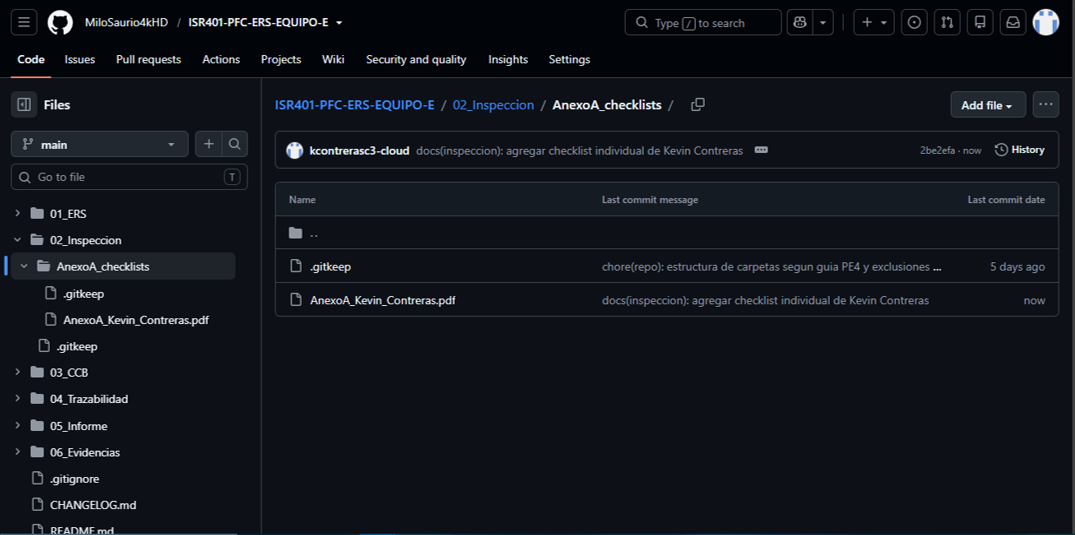
\includegraphics[width=0.85\textwidth]{figuras/commit_checklist_kevin.png}
		\caption{Evidencia del commit correspondiente al checklist individual del Inspector 2.
			Fuente: repositorio GitHub del equipo, carpeta
			\texttt{02\_Inspeccion/AnexoA\_checklists/}.}
		\label{fig:commit-kevin}
	\end{figure}
	
	\subsection{Acta de la reunión de inspección}
	
	\subsection{Registro consolidado de defectos}
	
	Los defectos registrados corresponden a contenido existente en el ERS Entrega 2A. No se incorporan
	identificadores de requisito inexistentes. La severidad se asigna según el impacto potencial sobre
	la interpretación, la privacidad, el comportamiento funcional o la trazabilidad.
	
	\begin{longtable}{C{1.0cm} L{2.0cm} L{4.6cm} L{1.9cm} L{1.7cm} L{1.8cm}}
		\caption{Registro de defectos consolidado (Anexo B)}\label{tab:defectos}\\
		\toprule
		\textbf{N.º} & \textbf{Sección} & \textbf{Descripción del defecto} & \textbf{Tipo} &
		\textbf{Severidad} & \textbf{Req. afectado} \\
		\midrule
		\endfirsthead
		\toprule
		\textbf{N.º} & \textbf{Sección} & \textbf{Descripción del defecto} & \textbf{Tipo} &
		\textbf{Severidad} & \textbf{Req. afectado} \\
		\midrule
		\endhead
		\bottomrule
		\endfoot
		D-01 & 1.5 &
		La visión general indica ``15 requisitos no funcionales'', pero el ERS vigente contiene RNF-01
		a RNF-16 y la clasificación posterior declara 16 RNF. & Consistencia & Menor & RNF-16 \\
		\addlinespace
		D-02 & 2.1, 2.2 y 2.4.2 &
		Se afirma que la veterinaria ``valida y certifica / verifica y certifica'' información médica,
		mientras el conflicto ``Validación documental limitada'' exige usar ``validación referencial''
		y no ``certificación clínica''. & Consistencia & Mayor & RF-09, RD-03 \\
		\addlinespace
		D-03 & 3.2.12 &
		RF-12 usa ``información requerida'' y ``documentación requerida'' sin fijar el mecanismo de
		identificación, aunque HU-09 reconoce que el mecanismo exacto sigue negociable. & Ambigüedad &
		Mayor & RF-12, HU-09 \\
		\addlinespace
		D-04 & 3.2.6 &
		RF-06 exige considerar raza, edad, salud, antecedentes genéticos, parentesco, comportamiento e
		historial médico; su criterio solo comprueba información comparativa y advertencia, sin
		comprobar los siete factores. & Completitud & Mayor & RF-06 \\
		\addlinespace
		D-05 & 2.2, 2.4.2 y 3.2.7 &
		El ERS declara ``Reporte de conversaciones sospechosas'' y mecanismos para reportar
		interacciones inadecuadas, pero RF-07 únicamente cubre envío y visualización de mensajes. &
		Completitud & Mayor & RF-07 \\
		\addlinespace
		D-06 & 3.2.7, 3.3.15 y CU-08 &
		RNF-15 y CU-08 asumen moderación automática, categorización y bloqueo de mensajes, pero RF-07
		no especifica funcionalmente ese procesamiento. & Consistencia & Mayor &
		RF-07, RNF-15, CU-08 \\
		\addlinespace
		D-07 & 3.5.1 y 3.3.17 / 4.7 &
		RD-01 solo menciona IA para compatibilidad e imágenes; el ERS identifica un tercer
		subcomponente de IA para moderación de mensajes. & Consistencia & Mayor & RD-01, RNF-15 \\
		\addlinespace
		D-08 & 3.2.17 &
		RF-17 rechaza imágenes que no cumplan ``criterios establecidos'', pero el RF no enumera esos
		criterios; RNF-14 sí menciona motivos concretos. & Ambigüedad & Mayor & RF-17, RNF-14 \\
		\addlinespace
		D-09 & 3.2.24 &
		RF-24 se titula ``cepa, lote y aplicador'', pero la descripción, entradas y criterio de
		verificación incluyen cepa/marca y aplicador, omitiendo el lote. & Consistencia & Mayor &
		RF-24 \\
		\addlinespace
		D-10 & 3.2.25 vs 3.3.16 &
		RF-25 exige que el aviso público muestre datos de contacto; RNF-16 exige ocultar por defecto
		el contacto directo a usuarios no autorizados. & Consistencia & Crítica &
		RF-25, RNF-16, RF-11 \\
		\addlinespace
		D-11 & 3.2.25 vs 3.1.2 / 3.3.16 &
		RF-25 recibe ``última ubicación conocida'' sin limitarla a zona aproximada; el ERS indica que
		la ubicación exacta no se almacena ni se muestra y RNF-16 exige radio aproximado
		$\geq$ 1 km. & Consistencia & Crítica & RF-25, RNF-16 \\
		\addlinespace
		D-12 & Apéndice D, TR-10 &
		La matriz enlaza RF-10 (recordatorios preventivos) con CU-12, pero CU-12 es ``Configurar
		privacidad médica'' y declara como RF asociados RF-11 y RF-03. & Trazabilidad & Mayor &
		RF-10, CU-12 \\
		\addlinespace
		D-13 & Apéndice D, TR-11 &
		La matriz enlaza RF-11 (privacidad) con CU-06 (compatibilidad de cruza), aunque el CU
		específico de privacidad es CU-12. & Trazabilidad & Mayor & RF-11, CU-06, CU-12 \\
		\addlinespace
		D-14 & Apéndice D, TR-33 &
		La matriz enlaza RF-20 (encuentros de socialización) con CU-08, pero CU-08 corresponde a
		comunicación y mensajería y no especifica la coordinación de encuentros. & Trazabilidad &
		Mayor & RF-20, CU-08 \\
		\addlinespace
		D-15 & Apéndice D, TR-38 &
		La matriz enlaza RF-25 (aviso de mascota extraviada) con CU-04, cuyo contenido es publicación
		de mascota en adopción; no existe un CU dedicado al aviso de extravío. & Trazabilidad & Mayor
		& RF-25, CU-04 \\
		\addlinespace
		D-16 & 3.3.6 &
		RNF-06 fija una coincidencia mínima del 85 \% con evaluaciones veterinarias, pero no define el
		tamaño ni la composición del ``conjunto representativo de casos de prueba''. &
		Verificabilidad & Mayor & RNF-06 \\
		\addlinespace
		D-17 & 3.3.7 &
		RNF-07 exige clasificar correctamente al menos el 95 \% de las imágenes ``según el tipo de
		fotografía esperado'', sin enumerar qué tipos son válidos o inválidos como referencia. &
		Verificabilidad & Mayor & RNF-07 \\
		\addlinespace
		D-18 & 3.3.11 &
		RNF-11 exige operar sin errores en Chrome, Firefox y Safari y en resoluciones de móvil y
		escritorio, pero no fija versiones ni resoluciones concretas de prueba. & Verificabilidad &
		Menor & RNF-11 \\
		\addlinespace
		D-19 & 3.3.13 / Apéndice D &
		RNF-13 se enlaza solo con RF-06, pero su verificación exige además evidencia de la
		explicación, medición de tiempo y encuesta de comprensión, sin enlaces explícitos en la
		matriz. & Trazabilidad & Menor & RNF-13, RF-06 \\
		\addlinespace
		D-20 & 3.3.14 / Apéndice D &
		RNF-14 se asocia a RF-17, pero la matriz no establece correspondencia clara entre el
		requisito, los criterios de aceptación y las pruebas de la explicación mostrada. &
		Trazabilidad & Menor & RNF-14, RF-17 \\
		\addlinespace
		D-21 & 3.3.3 &
		RNF-03 exige P95 $\leq$ 2 s con 100 usuarios concurrentes sin que el ERS declare la
		infraestructura ni el mecanismo de prueba que permitan ejecutar y medir esa carga. &
		Factibilidad & Mayor & RNF-03 \\
		\addlinespace
		D-22 & 3.3.6 &
		RNF-06 exige coincidencia $\geq$ 85 \% con evaluaciones de médicos veterinarios sin que exista
		un conjunto de casos evaluados por profesionales ni un procedimiento de evaluación declarado.
		& Factibilidad & Mayor & RNF-06 \\
		\addlinespace
		D-23 & 3.3.12 &
		RNF-12 fija P95 $\leq$ 3 s con 300 usuarios concurrentes, pero añade que no debe existir
		``degradación significativa'', expresión sin umbral cuantitativo propio. & Verificabilidad &
		Menor & RNF-12 \\
	\end{longtable}
	
	Resumen del registro: 23 defectos únicos consolidados. Los hallazgos D-01 a D-15 provienen del
	Inspector 2 y se concentran en los RF y las RD; los hallazgos D-16 a D-23 provienen del Inspector
	1 y se concentran en los RNF. Al aplicar la lectura por perspectivas, ambos conjuntos resultaron
	disjuntos y no fue necesario eliminar duplicados durante la consolidación. Por severidad se
	registran 2 defectos críticos, 16 mayores y 5 menores; por tipo, 7 de consistencia, 6 de
	trazabilidad, 4 de verificabilidad, 2 de ambigüedad, 2 de completitud y 2 de factibilidad. En
	total, 18 de 23 hallazgos (78,26 \%) requieren corrección prioritaria por estar clasificados como
	críticos o mayores.
	
	\subsection{Métricas de la inspección}
	
	Con el propósito de evaluar los resultados de la inspección Fagan realizada sobre el ERS de
	MundiPets se calcularon cinco métricas: densidad de defectos, distribución por tipo, distribución
	por severidad, tasa de detección por inspector y esfuerzo total. Todas se calculan sobre los 23
	defectos únicos consolidados en la Tabla \ref{tab:defectos}.
	
	\begin{table}[H]
		\centering
		\caption{Métricas de la inspección Fagan}
		\label{tab:metricas}
		\begin{tabular}{L{3.8cm} C{2.6cm} L{6.4cm}}
			\toprule
			\textbf{Métrica} & \textbf{Valor} & \textbf{Interpretación} \\
			\midrule
			Densidad de defectos & 1,92 def./página &
			Casi dos hallazgos por página en el tramo inspeccionado: la Sección 3 del ERS concentra
			el riesgo del documento y no admitía pasar a línea base sin revisión. \\
			\addlinespace
			Distribución por tipo & Consistencia 30,43 \% &
			El problema dominante no es la ausencia de requisitos, sino la contradicción entre
			secciones del mismo ERS. \\
			\addlinespace
			Distribución por severidad & Crítica + Mayor 78,26 \% &
			Los dos defectos críticos son ambos de privacidad sobre RF-25, el punto del ERS que
			debía corregirse antes de cualquier otra tarea. \\
			\addlinespace
			Tasa de detección por inspector & 2,88 def./h (global) &
			Las perspectivas asignadas produjeron conjuntos disjuntos: la lectura por perspectivas
			funcionó como mecanismo de cobertura, no solo de reparto. \\
			\addlinespace
			Esfuerzo total & 8,0 horas-persona &
			Ocho horas de preparación individual bastaron para detectar defectos que habrían llegado
			hasta el diseño si el ERS se hubiera aprobado sin inspección. \\
			\bottomrule
		\end{tabular}
	\end{table}
	
	\subsubsection{Densidad de defectos}
	
	La densidad de defectos permite determinar la cantidad de defectos encontrados en relación con el
	número de páginas efectivamente inspeccionadas:
	
	\begin{equation}
		D = \frac{\text{Número de defectos}}{\text{Número de páginas inspeccionadas}}
		\label{eq:densidad}
	\end{equation}
	
	La inspección se realizó sobre la Sección 3 del ERS, correspondiente a los requisitos específicos,
	que concentra los requisitos funcionales, no funcionales y las restricciones del sistema. Como
	denominador se emplea únicamente el número de páginas efectivamente inspeccionadas y no el total
	de páginas del documento. Con 23 defectos únicos consolidados y 12 páginas efectivamente
	inspeccionadas:
	
	\begin{equation*}
		D = \frac{23}{12} = 1{,}92~\text{defectos/página}
	\end{equation*}
	
	\textbf{Interpretación.} La densidad obtenida indica la concentración de defectos encontrada en el
	segmento del ERS sometido a inspección. Casi dos hallazgos por página muestran que la Sección 3
	requería atención prioritaria durante las actividades de corrección y validación, y justifica que
	el retrabajo se haya concentrado allí antes de establecer la línea base.
	
	\subsubsection{Distribución de defectos por tipo}
	
	Los 23 defectos consolidados fueron clasificados según el tipo de problema identificado. El
	porcentaje se calcula como el cociente entre la cantidad de defectos del tipo y el total de 23,
	multiplicado por 100.
	
	\begin{table}[H]
		\centering
		\caption{Distribución de defectos por tipo}
		\label{tab:dist-tipo}
		\begin{tabular}{L{4.0cm} C{2.4cm} C{2.4cm}}
			\toprule
			\textbf{Tipo de defecto} & \textbf{Cantidad} & \textbf{Porcentaje} \\
			\midrule
			Consistencia    & 7  & 30,43 \% \\
			Trazabilidad    & 6  & 26,09 \% \\
			Verificabilidad & 4  & 17,39 \% \\
			Ambigüedad      & 2  & 8,70 \% \\
			Completitud     & 2  & 8,70 \% \\
			Factibilidad    & 2  & 8,69 \% \\
			\midrule
			\textbf{Total}  & \textbf{23} & \textbf{100,00 \%} \\
			\bottomrule
		\end{tabular}
	\end{table}
	
	\begin{figure}[H]
		\centering
		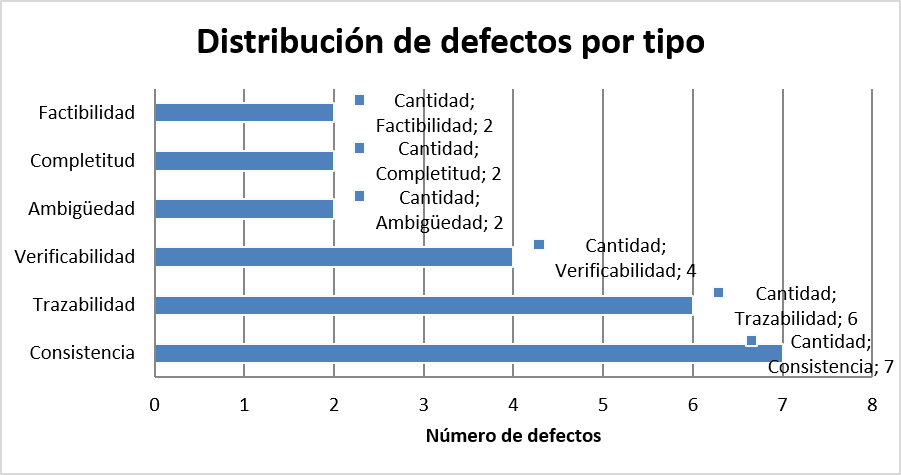
\includegraphics[width=0.86\textwidth]{figuras/metrica_tipo.png}
		\caption{Distribución de los 23 defectos consolidados por tipo.}
		\label{fig:metrica-tipo}
	\end{figure}
	
	\textbf{Interpretación.} El tipo con mayor presencia es la \textbf{consistencia}, con 7 defectos
	equivalentes al 30,43 \% del total, seguido de la \textbf{trazabilidad} con 6 defectos y el
	26,09 \%. Juntos superan la mitad de los hallazgos. Esto dice algo concreto sobre el ERS de
	MundiPets: los requisitos están individualmente redactados con detalle, pero el documento perdió
	sincronía entre sus secciones al crecer. Los defectos de verificabilidad y factibilidad, en
	cambio, se concentran íntegramente en los RNF, lo que indica que los umbrales numéricos se
	redactaron antes de decidir cómo se medirían.
	
	\subsubsection{Distribución de defectos por severidad}
	
	Los defectos también fueron clasificados según el nivel de impacto que representan para el
	proyecto.
	
	\begin{table}[H]
		\centering
		\caption{Distribución de defectos por severidad}
		\label{tab:dist-severidad}
		\begin{tabular}{L{4.0cm} C{2.4cm} C{2.4cm}}
			\toprule
			\textbf{Severidad} & \textbf{Cantidad} & \textbf{Porcentaje} \\
			\midrule
			Crítica         & 2  & 8,70 \% \\
			Mayor           & 16 & 69,56 \% \\
			Menor           & 5  & 21,74 \% \\
			\midrule
			\textbf{Total}  & \textbf{23} & \textbf{100,00 \%} \\
			\bottomrule
		\end{tabular}
	\end{table}
	
	\begin{figure}[H]
		\centering
		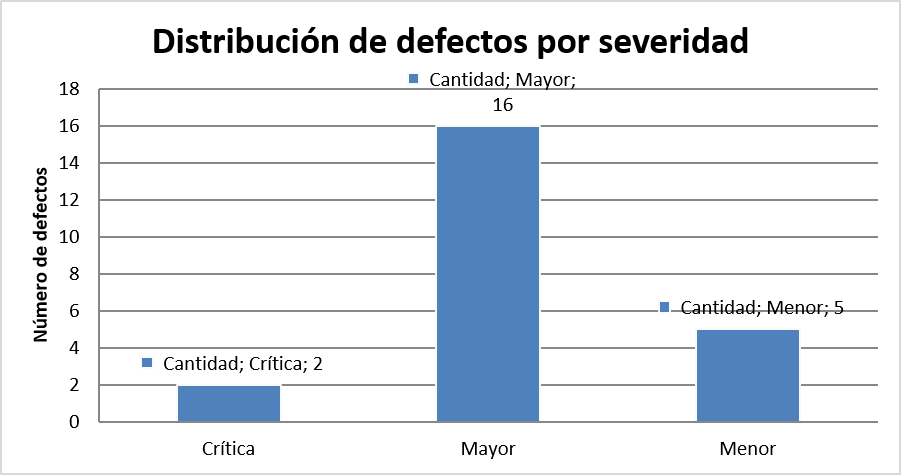
\includegraphics[width=0.80\textwidth]{figuras/metrica_severidad.png}
		\caption{Distribución de los 23 defectos consolidados por severidad.}
		\label{fig:metrica-severidad}
	\end{figure}
	
	\textbf{Interpretación.} El 78,26 \% de los defectos corresponde a severidades críticas o mayores,
	frente a un 21,74 \% de defectos menores. Los dos defectos críticos, D-10 y D-11, se refieren
	ambos al mismo requisito, RF-25, y ambos son contradicciones de privacidad frente a RNF-16: no se
	trata de dos incidencias dispersas, sino de un único requisito redactado sin consultar la
	restricción de protección de datos que el propio ERS declara. Esa concentración es la que justifica
	que RF-25 haya originado la RFC-03.
	
	\subsubsection{Tasa de detección por inspector}
	
	Para comparar el rendimiento de los inspectores se consideró la cantidad de defectos aportados al
	registro consolidado y las horas dedicadas a la preparación individual:
	
	\begin{equation}
		T = \frac{\text{Defectos detectados}}{\text{Horas empleadas}}
		\label{eq:tasa}
	\end{equation}
	
	\begin{table}[H]
		\centering
		\caption{Tasa de detección por inspector}
		\label{tab:tasa}
		\begin{tabular}{L{5.0cm} C{2.6cm} C{2.4cm} C{2.8cm}}
			\toprule
			\textbf{Inspector} & \textbf{Defectos} & \textbf{Horas} &
			\textbf{Tasa (def./h)} \\
			\midrule
			Contreras Chávez Kevin Germán (Inspector 2)  & 15 & 5,0 & 3,00 \\
			Viteri García Jonathan Enrique (Inspector 1) & 8  & 3,0 & 2,67 \\
			\midrule
			\textbf{Total} & \textbf{23} & \textbf{8,0} & \textbf{2,88} \\
			\bottomrule
		\end{tabular}
	\end{table}
	
	\textbf{Interpretación.} Kevin Contreras presenta la mayor cantidad de defectos aportados y la
	mayor tasa individual, con 3,00 defectos por hora, frente a 2,67 de Jonathan Viteri. La diferencia
	no refleja desigualdad de esfuerzo, sino de perspectiva: la consistencia y la trazabilidad se
	detectan comparando secciones y se acumulan rápido una vez identificado el patrón, mientras que la
	verificabilidad y la factibilidad exigen razonar sobre cada umbral por separado y rinden menos
	hallazgos por hora. Lo relevante es que ninguno de los 23 defectos fue encontrado por ambos: la
	asignación de perspectivas cumplió su función de ampliar cobertura.
	
	\subsubsection{Esfuerzo total de la inspección}
	
	El esfuerzo total corresponde a la suma de las horas dedicadas por los inspectores durante la
	preparación individual:
	
	\begin{equation*}
		E = 5{,}0 + 3{,}0 = 8{,}0~\text{horas-persona}
	\end{equation*}
	
	Al relacionar este esfuerzo con los 23 defectos encontrados se obtiene una productividad global de
	2,88 defectos por hora-persona.
	
	\textbf{Interpretación.} Ocho horas-persona de preparación permitieron detectar dos
	contradicciones críticas de privacidad, cuatro enlaces de trazabilidad incorrectos y un conjunto
	de umbrales no verificables. El costo del retrabajo declarado en las tres RFC asciende a 14
	horas-persona; detectar los mismos problemas después de haber diseñado clases y pruebas habría
	supuesto un esfuerzo considerablemente mayor. La relación entre ambos valores es el argumento
	cuantitativo a favor de mantener la inspección formal como paso previo a la línea base.
	
	% ═══════════════════════════════════════════════════════════════
	%  SECCIÓN 4 -- CORRECCIONES
	% ═══════════════════════════════════════════════════════════════
	\section{Correcciones aplicadas}
	\label{sec:correcciones}
	
	La tabla siguiente deja redactado el texto de corrección listo para trasladarlo a la versión
	resultante del ERS. La columna ``Texto ANTES'' reproduce el contenido relevante de la Entrega 2A;
	la columna ``Texto DESPUÉS'' alinea el artefacto con información ya existente en el propio ERS.
	Las decisiones de cambio que requieren CCB conservan la decisión registrada en el acta de la
	Sección \ref{sec:ccb}.
	
	\begin{longtable}{C{1.2cm} L{1.7cm} L{4.5cm} L{4.5cm} L{1.5cm}}
		\caption{Correcciones aplicadas a defectos críticos y mayores}\label{tab:correcciones}\\
		\toprule
		\textbf{Def.} & \textbf{Severidad} & \textbf{Texto ANTES} & \textbf{Texto DESPUÉS} &
		\textbf{Req.} \\
		\midrule
		\endfirsthead
		\toprule
		\textbf{Def.} & \textbf{Severidad} & \textbf{Texto ANTES} & \textbf{Texto DESPUÉS} &
		\textbf{Req.} \\
		\midrule
		\endhead
		\bottomrule
		\endfoot
		D-01 & Menor &
		``los 25 requisitos funcionales, los 15 requisitos no funcionales'' &
		``los 25 requisitos funcionales, los 16 requisitos no funcionales'' & RNF-16 \\
		\addlinespace
		D-02 & Mayor &
		``Veterinaria: valida y certifica la información médica y sanitaria\ldots'' /
		``verifiquen y certifiquen la información sanitaria y genética\ldots'' &
		``Veterinaria: realiza una validación referencial de la información médica y sanitaria
		registrada, sin constituir certificación clínica ni reemplazar una consulta veterinaria.'' &
		RF-09, RD-03 \\
		\addlinespace
		D-03 & Mayor &
		RF-12: ``mediante el registro y validación de la información requerida'' /
		``documentación requerida''. &
		``El sistema deberá verificar la identidad del usuario mediante sus datos básicos y un
		documento nacional de identidad legible antes de habilitar procesos de adopción o cruza; la
		verificación será rechazada cuando la documentación sea ilegible o incompleta.'' &
		RF-12, HU-09 \\
		\addlinespace
		D-04 & Mayor &
		``Seleccionar dos mascotas y comprobar que el sistema presenta la información comparativa
		junto con la advertencia orientativa.'' &
		``Seleccionar dos mascotas y comprobar que la evaluación considera raza, edad, estado de
		salud, antecedentes genéticos, parentesco, comportamiento e historial médico; verificar además
		la información comparativa y la advertencia de resultado orientativo.'' & RF-06 \\
		\addlinespace
		D-05 & Mayor &
		RF-07 solo permite ``comunicación \ldots mediante mensajes''. &
		Añadir: ``El sistema deberá permitir al usuario reportar mensajes o interacciones que
		considere spam, lenguaje ofensivo o acuerdos externos, registrando el motivo del reporte
		asociado a la conversación.'' & RF-07 \\
		\addlinespace
		D-06 & Mayor &
		RF-07 no describe la moderación que sí aparece en RNF-15 y CU-08. &
		Añadir a RF-07: ``Antes de entregar el mensaje, el sistema lo procesará mediante moderación
		automática; si se marca como inapropiado, mostrará la categoría detectada y bloqueará el envío
		conforme a RNF-15.'' & RF-07, RNF-15, CU-08 \\
		\addlinespace
		D-07 & Mayor &
		RD-01: ``\ldots IA para la evaluación de compatibilidad entre mascotas y la validación de
		imágenes\ldots'' &
		``El sistema deberá incorporar componentes de IA para evaluación de compatibilidad, validación
		de imágenes y moderación automática de mensajes, manteniendo los tres subcomponentes definidos
		en la arquitectura.'' & RD-01 \\
		\addlinespace
		D-08 & Mayor &
		RF-17: ``\ldots no cumplan con los criterios establecidos.'' &
		``\ldots validar si la imagen corresponde al tipo esperado y detectar, como mínimo, contenido
		inapropiado, imagen borrosa o tipo de fotografía incorrecto; cuando sea rechazada se mostrará
		el motivo conforme a RNF-14.'' & RF-17, RNF-14 \\
		\addlinespace
		D-09 & Mayor &
		RF-24 omite ``lote'' en descripción, entradas y criterio. &
		Descripción, entradas y criterio deben incluir ``número de lote'' junto con cepa o marca,
		aplicador y fecha; el criterio comprobará que los tres datos de trazabilidad aparezcan en el
		carnet. & RF-24 \\
		\addlinespace
		D-10 & Crítica &
		RF-25: ``aviso público \ldots incluyendo \ldots datos de contacto'' y criterio
		``visible \ldots con los datos de contacto''. &
		``El aviso será público, pero los datos de contacto directo permanecerán ocultos por defecto.
		Solo se mostrarán cuando el propietario autorice expresamente su visibilidad mediante RF-11;
		en caso contrario se conservará la protección definida en RNF-16.'' &
		RF-25, RF-11, RNF-16 \\
		\addlinespace
		D-11 & Crítica &
		RF-25, entrada: ``última ubicación conocida''. &
		Sustituir por ``zona aproximada de última ubicación conocida (radio $\geq$ 1 km)''; el aviso
		no almacenará ni mostrará la dirección exacta, en coherencia con RNF-16. & RF-25, RNF-16 \\
		\addlinespace
		D-12 & Mayor & TR-10: RF-10 $\rightarrow$ CU-12. &
		Eliminar el enlace RF-10 $\rightarrow$ CU-12 y registrar ``sin CU específico en la versión
		inspeccionada''; crear y enlazar un CU de recordatorios solo si el equipo lo aprueba en la
		actualización de trazabilidad. & RF-10, CU-12 \\
		\addlinespace
		D-13 & Mayor & TR-11: RF-11 $\rightarrow$ CU-06. &
		TR-11: RF-11 $\rightarrow$ CU-12 (Configurar privacidad médica), manteniendo HU-08, CA-08 y
		MU-08. & RF-11, CU-12 \\
		\addlinespace
		D-14 & Mayor & TR-33: RF-20 $\rightarrow$ CU-08. &
		Eliminar RF-20 $\rightarrow$ CU-08 y registrar ``sin CU específico en la versión
		inspeccionada''; CU-08 se mantiene únicamente para mensajería. & RF-20, CU-08 \\
		\addlinespace
		D-15 & Mayor & TR-38: RF-25 $\rightarrow$ CU-04. &
		Eliminar RF-25 $\rightarrow$ CU-04 y registrar ``sin CU específico en la versión
		inspeccionada''; CU-04 conserva su propósito de publicación en adopción. & RF-25, CU-04 \\
	\end{longtable}
	
	\subsection{Defectos menores no corregidos y su justificación}
	
	No quedan defectos menores pendientes en el alcance cubierto por el Inspector 2. El defecto D-01,
	aunque fue clasificado como menor, se corrige porque el cambio es directo y evita que la
	introducción del ERS contradiga el inventario vigente de 16 RNF. Los demás hallazgos se incorporan
	a la Tabla \ref{tab:correcciones} por su severidad crítica o mayor.
	
	% ═══════════════════════════════════════════════════════════════
	%  SECCIÓN 5 -- CCB
	% ═══════════════════════════════════════════════════════════════
	\section{Gestión del cambio y Change Control Board}
	\label{sec:ccb}
	
	\subsection{RFC-01 -- Cambio de alcance}
	
	Origen verificable: conflicto ``Comunicación inadecuada entre usuarios'' de la Sección 2.4.2 y
	función de producto ``Reporte de conversaciones sospechosas'' de la Sección 2.2 del ERS. La RFC no
	crea un problema nuevo: formaliza una necesidad ya documentada en el ERS que actualmente no tiene
	un RF operativo completo.
	
	\begin{longtable}{L{4.0cm} L{9.5cm}}
		\caption{Formulario RFC-01 -- Cambio de alcance}\label{tab:rfc01}\\
		\toprule
		\textbf{Campo} & \textbf{Contenido} \\
		\midrule
		\endfirsthead
		\toprule
		\textbf{Campo} & \textbf{Contenido} \\
		\midrule
		\endhead
		\bottomrule
		\endfoot
		ID / Fecha / Solicitante &
		RFC-01 / 08/08/2026 / Contreras Chávez Kevin Germán \\
		\addlinespace
		Requisito afectado &
		RF-07 -- Sistema de mensajería entre usuarios. Se propone incorporar un requisito funcional
		nuevo o ampliar RF-07 para cubrir el reporte de interacciones inadecuadas. \\
		\addlinespace
		Descripción del cambio &
		Incorporar la capacidad de reportar mensajes o interacciones consideradas spam, lenguaje
		ofensivo o acuerdos externos, registrando el motivo del reporte asociado a la conversación. \\
		\addlinespace
		Justificación de negocio &
		El ERS reconoce el conflicto ``Comunicación inadecuada entre usuarios'', cuyo impacto es la
		disminución de confianza y el uso inadecuado de la plataforma. La estrategia documentada exige
		reglas, advertencias y mecanismos básicos para reportar interacciones inadecuadas. Además, la
		Sección 2.2 ya declara el reporte de conversaciones sospechosas como función del producto. \\
		\addlinespace
		Requisitos impactados (desde la matriz) &
		RF-07 y RNF-15. La moderación automática y la explicación de la categoría detectada deben
		permanecer coherentes con el reporte manual del usuario. \\
		\addlinespace
		Artefactos impactados (CU, clases, pruebas) &
		CU-08 Gestionar comunicación entre usuarios; clase \texttt{Mensaje}; componente Mensajería.
		Crear caso de prueba para reportar una interacción y comprobar que el motivo quede asociado a
		la conversación. \\
		\addlinespace
		Costo estimado / Riesgo &
		Estimación académica: 6 horas-persona para ajuste de requisito, CU, trazabilidad y prueba.
		Riesgo medio: duplicar responsabilidades entre moderación automática y reporte manual si no se
		separan ambos flujos. \\
		\addlinespace
		Alternativas evaluadas &
		(A) Incorporar el reporte manual dentro del flujo de mensajería (recomendada).
		(B) Mantener únicamente moderación automática: no cubre el mecanismo de reporte solicitado en
		el conflicto.
		(C) Diferir la función: conserva una brecha entre el alcance declarado y el RF. \\
		\addlinespace
		Recomendación técnica &
		Aprobar con la condición de distinguir dos eventos: moderación automática antes del envío y
		reporte manual posterior o por iniciativa del usuario. Ambos deben enlazarse a RF-07 y CU-08
		sin atribuir a la plataforma funciones clínicas ni administrativas no definidas. \\
		\addlinespace
		Decisión del CCB / Justificación / Responsable / Plazo &
		\textbf{Aprobado con condiciones.} El CCB aprueba incorporar el mecanismo de reporte manual de
		mensajes e interacciones inadecuadas dentro del flujo de mensajería, debido a que el ERS
		identifica la ``Comunicación inadecuada entre usuarios'' como un conflicto que puede afectar
		la confianza y el uso adecuado de la plataforma. Como condición, el reporte manual deberá
		diferenciarse de la moderación automática ya contemplada en el sistema, evitando duplicidad de
		funciones. Responsable: Contreras Chávez Kevin Germán, con revisión de Fuertes Arraes Edson
		Daniel. Plazo: 24 horas posteriores a la aprobación del CCB y antes de establecer la línea
		base \texttt{baseline-v1.1}. \\
	\end{longtable}
	
	\subsection{RFC-02 -- Cambio de calidad (RNF)}
	
	Origen verificable: defectos D-21 y D-23 del registro consolidado, que señalan que el umbral de
	RNF-03 se fijó sin declarar la infraestructura ni el mecanismo de prueba que permitan medirlo. La
	RFC ajusta el umbral a un valor comprobable con los recursos del proyecto, sin eliminar el
	objetivo cuantitativo. El requisito se corresponde con la característica de eficiencia de
	desempeño del modelo de calidad de producto de ISO/IEC 25010 \cite{iso25010}.
	
	\begin{longtable}{L{4.0cm} L{9.5cm}}
		\caption{Formulario RFC-02 -- Cambio de calidad}\label{tab:rfc02}\\
		\toprule
		\textbf{Campo} & \textbf{Contenido} \\
		\midrule
		\endfirsthead
		\toprule
		\textbf{Campo} & \textbf{Contenido} \\
		\midrule
		\endhead
		\bottomrule
		\endfoot
		ID / Fecha / Solicitante &
		RFC-02 / 08/08/2026 / Viteri García Jonathan Enrique \\
		\addlinespace
		Requisito afectado & RNF-03 -- Tiempo de respuesta. \\
		\addlinespace
		Descripción del cambio &
		Modificar el umbral de tiempo de respuesta de RNF-03 manteniendo el uso del percentil 95 (P95)
		como mecanismo de medición. El nuevo objetivo establece un P95 máximo de \textbf{3 segundos}
		bajo una carga de \textbf{100 usuarios concurrentes}. \\
		\addlinespace
		Justificación de negocio &
		El cambio busca establecer un umbral de rendimiento que pueda ser alcanzado y comprobado con
		la infraestructura disponible, manteniendo un tiempo de respuesta adecuado para los usuarios
		de MundiPets. El defecto D-21 documenta que el valor anterior no era factible de verificar con
		los recursos declarados en el ERS. \\
		\addlinespace
		Valor anterior / Valor propuesto &
		Anterior: P95 $\leq$ 2 segundos con 100 usuarios concurrentes.
		Propuesto: P95 $\leq$ 3 segundos con 100 usuarios concurrentes. \\
		\addlinespace
		Requisitos impactados (desde la matriz) &
		RNF-03 y RNF-12, además de los RF sometidos a las pruebas de rendimiento (RF-04, RF-06 y
		RF-17, por ser los de mayor costo computacional según el diagrama de componentes). El efecto
		cruzado relevante es que relajar RNF-03 amplía el margen de cómputo disponible para el
		componente de IA, lo que favorece la exactitud exigida por RNF-06 y RNF-07. \\
		\addlinespace
		Artefactos impactados (CU, clases, pruebas) &
		ERS, matriz de trazabilidad, historias de usuario, criterios de aceptación y casos de prueba
		de rendimiento. \\
		\addlinespace
		Costo estimado / Riesgo &
		Estimación académica: 3 horas-persona. Riesgo medio: reducir la exigencia de rendimiento puede
		afectar la percepción de fluidez si el valor real se acerca sistemáticamente al nuevo techo.
		\\
		\addlinespace
		Alternativas evaluadas &
		(A) Mantener P95 $\leq$ 2 s y ampliar la infraestructura: descartada por presupuesto cero.
		(B) Eliminar el umbral numérico: descartada por hacer el requisito no verificable.
		(C) Elevar el umbral a 3 s conservando el P95 y la carga de 100 usuarios: recomendada, porque
		mantiene el objetivo medible y lo vuelve alcanzable. \\
		\addlinespace
		Recomendación técnica &
		Aprobar el cambio de manera condicionada a la ejecución de pruebas de carga con 100 usuarios
		concurrentes y a la actualización de los artefactos relacionados. \\
		\addlinespace
		Decisión del CCB / Justificación / Responsable / Plazo &
		\textbf{Aprobado con condiciones.} El CCB considera que el nuevo umbral mantiene un objetivo
		de rendimiento medible y permite una mayor factibilidad de implementación. La aprobación queda
		condicionada a la actualización de la documentación y a la comprobación del nuevo umbral
		mediante pruebas de rendimiento con 100 usuarios concurrentes. Responsable: Contreras Chávez
		Kevin Germán. Plazo: 3 días posteriores a la aprobación de la RFC. Versión resultante del ERS:
		v1.1. \\
	\end{longtable}
	
	\subsection{RFC-03 -- Cambio por restricción o normativa}
	
	Origen verificable: RF-25, RF-11, RNF-16, RD-04 y la trazabilidad legal del ERS. El cambio se
	fundamenta en las obligaciones que el propio documento asigna a la LOPDP: minimización y seguridad
	(RL-05, Art. 10 lit. e y j) y protección de datos desde el diseño y por defecto (RL-08, Art. 39).
	
	\begin{longtable}{L{4.0cm} L{9.5cm}}
		\caption{Formulario RFC-03 -- Cambio por restricción o normativa}\label{tab:rfc03}\\
		\toprule
		\textbf{Campo} & \textbf{Contenido} \\
		\midrule
		\endfirsthead
		\toprule
		\textbf{Campo} & \textbf{Contenido} \\
		\midrule
		\endhead
		\bottomrule
		\endfoot
		ID / Fecha / Solicitante &
		RFC-03 / 08/08/2026 / Contreras Chávez Kevin Germán \\
		\addlinespace
		Requisito afectado & RF-25 -- Publicar aviso de mascota extraviada. \\
		\addlinespace
		Descripción del cambio &
		Modificar RF-25 para que el aviso público utilice zona aproximada de última ubicación
		(radio $\geq$ 1 km) y mantenga ocultos por defecto los datos de contacto directo. La
		visibilidad del contacto solo podrá habilitarse mediante autorización expresa del propietario
		conforme a RF-11. \\
		\addlinespace
		Justificación de negocio &
		La versión inspeccionada ordena publicar los datos de contacto y recibe la ``última ubicación
		conocida'', pero RNF-16 exige ocultar por defecto la ubicación exacta y el contacto directo.
		Mantener ambos textos sin corrección crea una contradicción con la minimización y la
		protección por defecto declaradas en el propio ERS. \\
		\addlinespace
		Requisitos impactados (desde la matriz) &
		RF-25, RF-11, RNF-16 y RD-04. También debe revisarse la fila TR-38, porque actualmente enlaza
		RF-25 con CU-04, un caso de uso de adopción. \\
		\addlinespace
		Artefactos impactados (CU, clases, pruebas) &
		Clase \texttt{AvisoExtraviado}; reglas de privacidad aplicadas al perfil y al aviso; matriz
		TR-38; caso de prueba de aviso público sin exposición de contacto ni ubicación exacta. \\
		\addlinespace
		Costo estimado / Riesgo &
		Estimación académica: 5 horas-persona para ajuste de especificación, trazabilidad y pruebas.
		Riesgo alto si no se corrige: exposición de datos personales y contradicción verificable entre
		RF-25 y RNF-16. \\
		\addlinespace
		Alternativas evaluadas &
		(A) Mostrar contacto y ubicación exactos públicamente: rechazada por conflicto con RNF-16.
		(B) Ocultar todo dato de localización: reduce la utilidad del aviso.
		(C) Mostrar zona aproximada y contacto condicionado a autorización: recomendada por equilibrar
		localización y privacidad. \\
		\addlinespace
		Recomendación técnica &
		Aprobar el cambio normativo con la redacción propuesta y corregir TR-38. La prueba debe
		ejecutarse desde una cuenta sin autorización específica y comprobar que no aparezcan dirección
		exacta ni contacto directo. \\
		\addlinespace
		Decisión del CCB / Justificación / Responsable / Plazo &
		\textbf{Aprobado.} El CCB aprueba modificar RF-25 para que el aviso de mascota extraviada
		muestre únicamente una zona aproximada de la última ubicación y mantenga ocultos por defecto
		los datos de contacto directo. La decisión se justifica porque la redacción actual entra en
		conflicto con RNF-16 y RD-04, además de la configuración de privacidad contemplada en RF-11.
		También se deberá corregir la trazabilidad asociada a TR-38 para evitar una relación
		incorrecta con un caso de uso no correspondiente. Responsable: Contreras Chávez Kevin Germán,
		encargado de actualizar RF-25 y la matriz de trazabilidad, con revisión de Fuertes Arraes
		Edson Daniel. Plazo: 24 horas posteriores a la aprobación del CCB y antes de establecer la
		línea base \texttt{baseline-v1.1}. \\
	\end{longtable}
	
	\subsection{Acta del CCB}
	\label{sec:acta-ccb}
	
	\noindent\textbf{Proyecto:} MundiPets \quad\textbf{Acta N.º:} CCB-01 \quad
	\textbf{Fecha:} 09/08/2026\\
	\textbf{Hora de inicio:} 10:00 \quad \textbf{Hora de finalización:} 11:15 \quad
	\textbf{Modalidad:} reunión virtual
	
	\subsubsection{Integrantes y roles}
	
	\begin{table}[H]
		\centering
		\caption{Integrantes del Change Control Board}
		\label{tab:ccb-roles}
		\begin{tabular}{L{6.0cm} L{5.5cm}}
			\toprule
			\textbf{Integrante} & \textbf{Rol en el CCB} \\
			\midrule
			Fuertes Arraes Edson Daniel      & Presidente del CCB \\
			Contreras Chávez Kevin Germán    & Analista del CCB \\
			Viteri García Jonathan Enrique   & Representante del cliente \\
			\bottomrule
		\end{tabular}
	\end{table}
	
	El CCB se reunió con el propósito de analizar las tres solicitudes de cambio registradas para el
	proyecto MundiPets y determinar su aprobación, rechazo o aplazamiento, considerando los impactos
	técnicos, funcionales, de calidad, costo y trazabilidad.
	
	\subsubsection{Deliberación de RFC-01 -- Cambio de alcance}
	
	\textbf{Tipo:} cambio de alcance.
	
	\textbf{Descripción:} ampliar RF-07 para incorporar el reporte manual de mensajes e interacciones
	consideradas spam, lenguaje ofensivo o acuerdos externos, registrando el motivo del reporte
	asociado a la conversación.
	
	\textbf{Argumento del Presidente:} la funcionalidad puede aportar valor al sistema, pero debe
	analizarse si su implementación afecta el alcance establecido y los recursos disponibles. Señaló
	que el equipo dispone de 8 horas de práctica y que 6 horas-persona representan una fracción
	relevante del presupuesto de esfuerzo.
	
	\textbf{Argumento del Analista:} el cambio implica modificar varios artefactos del proyecto,
	principalmente RF-07, CU-08, la clase \texttt{Mensaje} y el componente de Mensajería, además de
	crear el caso de prueba correspondiente. Advirtió que el reporte manual debe separarse
	explícitamente de la moderación automática ya prevista en RNF-15 para no duplicar
	responsabilidades.
	
	\textbf{Argumento del Representante del cliente:} la funcionalidad resulta conveniente porque el
	propio ERS ya declara el reporte de conversaciones sospechosas como función de producto en la
	Sección 2.2; no incorporarla mantendría una brecha entre el alcance declarado y el requisito
	operativo.
	
	\textbf{Decisión: aprobado con condiciones.}
	
	\textbf{Justificación:} el CCB considera que la funcionalidad cierra una brecha ya documentada en
	el ERS, pero su incorporación debe realizarse sin afectar los requisitos Must existentes ni
	comprometer las actividades prioritarias del proyecto. Como condición, el reporte manual deberá
	diferenciarse de la moderación automática.
	
	\textbf{Acciones:} ampliar RF-07 en el ERS; crear la historia de usuario y sus criterios de
	aceptación de mensajería reportable; actualizar la matriz de trazabilidad; incorporar la
	funcionalidad al tablero CASE.
	
	\textbf{Responsable:} Contreras Chávez Kevin Germán. \quad \textbf{Plazo:} 24 horas.
	
	\subsubsection{Deliberación de RFC-02 -- Cambio de calidad}
	
	\textbf{Tipo:} cambio de calidad. \quad \textbf{Requisito afectado:} RNF-03 -- Tiempo de
	respuesta.
	
	\textbf{Descripción:} modificación del objetivo de rendimiento de P95 $\leq$ 2 segundos a
	P95 $\leq$ 3 segundos con 100 usuarios concurrentes.
	
	\textbf{Argumento del Presidente:} el cambio reduce la exigencia original de rendimiento, por lo
	que debe comprobarse que el nuevo valor continúe proporcionando una experiencia adecuada para los
	usuarios y que no se convierta en un precedente para relajar otros RNF.
	
	\textbf{Argumento del Analista:} el cambio es técnicamente medible y puede verificarse mediante
	pruebas de carga. Señaló además el efecto cruzado favorable: el margen adicional de cómputo
	beneficia la exactitud exigida por RNF-06 y RNF-07, que el Inspector 1 ya había marcado como
	dudosa en factibilidad. Será necesario actualizar el ERS, la matriz de trazabilidad y los casos de
	prueba relacionados.
	
	\textbf{Argumento del Representante del cliente:} el cambio es aceptable siempre que el tiempo de
	respuesta continúe siendo razonable y se compruebe mediante pruebas objetivas, no por estimación.
	
	\textbf{Decisión: aprobado con condiciones.}
	
	\textbf{Justificación:} el nuevo umbral mejora la factibilidad de cumplimiento sin eliminar el
	objetivo cuantificable de rendimiento. La aprobación queda condicionada a la realización de
	pruebas con 100 usuarios concurrentes y al cumplimiento de un P95 máximo de 3 segundos.
	
	\textbf{Acciones:} actualizar RNF-03 en el ERS; actualizar los criterios de aceptación afectados;
	actualizar la matriz de trazabilidad; modificar los casos de prueba de rendimiento; ejecutar las
	pruebas de carga correspondientes.
	
	\textbf{Responsable:} Contreras Chávez Kevin Germán. \quad \textbf{Plazo:} 3 días.
	
	\subsubsection{Deliberación de RFC-03 -- Cambio por restricción o normativa}
	
	\textbf{Tipo:} cambio por restricción. \quad \textbf{Requisito afectado:} RF-25 -- Publicar aviso
	de mascota extraviada.
	
	\textbf{Descripción:} el aviso público deberá utilizar zona aproximada de última ubicación
	(radio $\geq$ 1 km) y mantener ocultos por defecto los datos de contacto directo, habilitándolos
	solo mediante autorización expresa del propietario conforme a RF-11.
	
	\textbf{Argumento del Presidente:} las restricciones relacionadas con el manejo de información
	deben considerarse antes de incorporar cambios que puedan afectar datos de usuarios o mascotas.
	Recordó que D-10 y D-11, los dos únicos defectos críticos de la inspección, corresponden a este
	requisito.
	
	\textbf{Argumento del Analista:} la incorporación de la restricción requiere revisar los
	requisitos relacionados con privacidad, almacenamiento y acceso a la información, y corregir la
	fila TR-38 de la matriz, que actualmente enlaza RF-25 con un caso de uso de adopción. El riesgo de
	no corregir es alto: exposición de datos personales y contradicción verificable con RNF-16 y
	RD-04.
	
	\textbf{Argumento del Representante del cliente:} la protección de la información es necesaria
	para mantener la confianza de los usuarios; no obstante, pidió constancia de que ocultar la
	ubicación exacta no inutilice el aviso de extravío, motivo por el que se conserva la zona
	aproximada en lugar de suprimir toda referencia geográfica.
	
	\textbf{Decisión: aprobado.}
	
	\textbf{Justificación:} el CCB determinó que la restricción es necesaria para resolver una
	contradicción interna del ERS y para cumplir las obligaciones de minimización y protección por
	defecto que el propio documento asigna a la LOPDP, sin representar un impacto significativo sobre
	el alcance funcional.
	
	\textbf{Acciones:} modificar RF-25 en el ERS; revisar los requisitos relacionados con privacidad;
	corregir la fila TR-38 de la matriz de trazabilidad; revisar los criterios de aceptación
	afectados; registrar el cambio en el historial de versiones.
	
	\textbf{Responsable:} Contreras Chávez Kevin Germán. \quad \textbf{Plazo:} 24 horas.
	
	\subsubsection{Resumen de decisiones}
	
	\begin{table}[H]
		\centering
		\caption{Resumen de decisiones del CCB}
		\label{tab:ccb-resumen}
		\begin{tabular}{L{1.6cm} L{3.4cm} L{3.4cm} L{3.0cm} C{1.6cm}}
			\toprule
			\textbf{RFC} & \textbf{Tipo} & \textbf{Decisión} & \textbf{Responsable} &
			\textbf{Plazo} \\
			\midrule
			RFC-01 & Cambio de alcance & Aprobado con condiciones & Kevin Contreras & 24 h \\
			RFC-02 & Cambio de calidad & Aprobado con condiciones & Kevin Contreras & 3 días \\
			RFC-03 & Restricción o normativa & Aprobado & Kevin Contreras & 24 h \\
			\bottomrule
		\end{tabular}
	\end{table}
	
	\subsubsection{Impacto sobre la configuración}
	
	Las RFC aprobadas deberán incorporarse a los artefactos afectados del proyecto. En particular
	deberán actualizarse el ERS, la matriz de trazabilidad, las historias de usuario, los criterios de
	aceptación, los casos de prueba, el tablero CASE y el historial de cambios. El costo total
	comprometido asciende a 14 horas-persona (6 de RFC-01, 3 de RFC-02 y 5 de RFC-03).
	
	\subsubsection{Acciones y seguimiento}
	
	\begin{table}[H]
		\centering
		\caption{Acciones de seguimiento acordadas por el CCB}
		\label{tab:ccb-seguimiento}
		\begin{tabular}{L{5.6cm} L{3.4cm} C{1.8cm} C{2.0cm}}
			\toprule
			\textbf{Acción} & \textbf{Responsable} & \textbf{Plazo} & \textbf{Estado} \\
			\midrule
			Ampliar RF-07 en el ERS (RFC-01)          & Kevin Contreras  & 24 h   & Pendiente \\
			Actualizar RNF-03 (RFC-02)                & Kevin Contreras  & 3 días & Pendiente \\
			Ejecutar pruebas de rendimiento           & Kevin Contreras  & 3 días & Pendiente \\
			Modificar RF-25 y corregir TR-38 (RFC-03) & Kevin Contreras  & 24 h   & Pendiente \\
			Actualizar la matriz de trazabilidad      & Kevin Contreras  & 3 días & Pendiente \\
			Actualizar el tablero CASE                & Jonathan Viteri  & 3 días & Pendiente \\
			Registrar los cambios en el CHANGELOG     & Edson Fuertes    & 3 días & Pendiente \\
			\bottomrule
		\end{tabular}
	\end{table}
	
	\subsubsection{Versión resultante y cierre de la reunión}
	
	Como resultado de las decisiones tomadas, las modificaciones aprobadas deberán incorporarse en la
	versión controlada \textbf{ERS v1.1}, manteniendo la trazabilidad entre los requisitos modificados
	y los artefactos relacionados y registrando las modificaciones en el historial de cambios del
	documento.
	
	Una vez analizadas las tres solicitudes de cambio, los integrantes del CCB estuvieron de acuerdo
	con las decisiones registradas en la presente acta. La sesión finalizó a las 11:15 del 09/08/2026.
	
	\vspace{0.4cm}
	\noindent\textbf{Firmas:}
	
	\vspace{0.6cm}
	\noindent
	\begin{minipage}[t]{0.32\textwidth}
		\centering
		\rule{4.2cm}{0.4pt}\\
		\small Fuertes Arraes Edson Daniel\\
		\textit{Presidente del CCB}
	\end{minipage}%
	\begin{minipage}[t]{0.32\textwidth}
		\centering
		\rule{4.2cm}{0.4pt}\\
		\small Contreras Chávez Kevin Germán\\
		\textit{Analista del CCB}
	\end{minipage}%
	\begin{minipage}[t]{0.32\textwidth}
		\centering
		\rule{4.2cm}{0.4pt}\\
		\small Viteri García Jonathan Enrique\\
		\textit{Representante del cliente}
	\end{minipage}
	
	\subsection{Versión resultante del ERS}
	
	% ═══════════════════════════════════════════════════════════════
	%  SECCIÓN 6 -- TRAZABILIDAD CASE
	% ═══════════════════════════════════════════════════════════════
	\section{Trazabilidad en herramienta CASE}
	
	\subsection{Estructura del tablero}
	
	Para la gestión de requisitos de MundiPets se utiliza Jira, por las razones argumentadas en la
	Sección \ref{sec:recomendacion}. El tablero se organiza mediante la jerarquía
	\textbf{Epic $\rightarrow$ Story $\rightarrow$ Sub-task}, que permite agrupar los requisitos
	funcionales por áreas del sistema y descomponer cada requisito en actividades concretas de
	trabajo.
	
	El ERS de MundiPets contiene 25 requisitos funcionales, desde RF-01 hasta RF-25, con prioridades
	asignadas mediante MoSCoW. Para el tablero se establecieron cinco Epics que agrupan los requisitos
	de acuerdo con la funcionalidad principal que representan.
	
	\begin{longtable}{L{1.5cm} L{1.5cm} L{7.6cm} L{1.6cm}}
		\caption{Estructura Epic $\rightarrow$ Story del tablero CASE de MundiPets}
		\label{tab:tablero}\\
		\toprule
		\textbf{Epic} & \textbf{Story} & \textbf{Requisito} & \textbf{Prioridad} \\
		\midrule
		\endfirsthead
		\toprule
		\textbf{Epic} & \textbf{Story} & \textbf{Requisito} & \textbf{Prioridad} \\
		\midrule
		\endhead
		\bottomrule
		\endfoot
		\multicolumn{4}{l}{\textbf{EPIC-01 -- Gestión de mascotas y perfiles}} \\
		& ST-01 & RF-01 -- Registrar mascota & Must \\
		& ST-02 & RF-02 -- Gestionar historial médico de la mascota & Must \\
		& ST-03 & RF-03 -- Consultar perfil completo de una mascota & Must \\
		& ST-04 & RF-13 -- Registrar publicaciones de mascotas & Must \\
		& ST-05 & RF-14 -- Gestionar carnet de vacunación & Must \\
		& ST-06 & RF-16 -- Gestionar antecedentes genéticos y parentesco & Must \\
		& ST-07 & RF-21 -- Registrar el identificador de microchip & Should \\
		\addlinespace
		\multicolumn{4}{l}{\textbf{EPIC-02 -- Adopción y seguimiento}} \\
		& ST-08 & RF-04 -- Buscar y filtrar mascotas & Should \\
		& ST-09 & RF-05 -- Gestionar solicitudes de adopción & Must \\
		& ST-10 & RF-18 -- Gestionar el flujo de solicitud de adopción por etapas & Must \\
		& ST-11 & RF-22 -- Dar seguimiento post-adopción & Must \\
		& ST-12 & RF-25 -- Publicar aviso de mascota extraviada & Could \\
		\addlinespace
		\multicolumn{4}{l}{\textbf{EPIC-03 -- Cruza y compatibilidad}} \\
		& ST-13 & RF-06 -- Evaluar compatibilidad entre mascotas para cruza & Must \\
		& ST-14 & RF-08 -- Gestionar solicitudes de cruza & Must \\
		& ST-15 & RF-19 -- Validar certificados veterinarios antes de habilitar la cruza & Should \\
		& ST-16 & RF-23 -- Emitir alertas de riesgo sanitario o físico & Must \\
		\addlinespace
		\multicolumn{4}{l}{\textbf{EPIC-04 -- Usuarios, comunicación y seguridad}} \\
		& ST-17 & RF-07 -- Sistema de mensajería entre usuarios & Could \\
		& ST-18 & RF-11 -- Administrar la privacidad de la información & Must \\
		& ST-19 & RF-12 -- Verificar la identidad de los usuarios & Must \\
		& ST-20 & RF-20 -- Coordinar encuentros de socialización supervisados & Could \\
		\addlinespace
		\multicolumn{4}{l}{\textbf{EPIC-05 -- Salud, validación y trazabilidad veterinaria}} \\
		& ST-21 & RF-09 -- Validar la información médica de una mascota & Must \\
		& ST-22 & RF-10 -- Gestionar recordatorios de controles preventivos & Should \\
		& ST-23 & RF-15 -- Consultar el historial de procesos de adopción y cruza & Could \\
		& ST-24 & RF-17 -- Validar imágenes & Should \\
		& ST-25 & RF-24 -- Registrar trazabilidad de cepa, lote y aplicador de cada vacuna &
		Should \\
	\end{longtable}
	
	\subsubsection{Sub-tasks}
	
	Las Stories que contienen criterios de aceptación se descomponen en actividades concretas. Se
	seleccionaron cinco Stories y se establecieron dos Sub-tasks para cada una.
	
	\begin{longtable}{L{1.5cm} L{4.9cm} L{6.8cm}}
		\caption{Sub-tasks derivadas de los criterios de aceptación}
		\label{tab:subtasks}\\
		\toprule
		\textbf{Story} & \textbf{Criterio de aceptación} & \textbf{Sub-tasks} \\
		\midrule
		\endfirsthead
		\toprule
		\textbf{Story} & \textbf{Criterio de aceptación} & \textbf{Sub-tasks} \\
		\midrule
		\endhead
		\bottomrule
		\endfoot
		ST-01 \newline (RF-01) &
		Registrar una mascota con datos válidos y comprobar que el perfil queda almacenado y puede
		consultarse posteriormente. &
		(a) Implementar el formulario de registro con los campos requeridos.
		(b) Verificar el almacenamiento y la consulta posterior del perfil registrado. \\
		\addlinespace
		ST-05 \newline (RF-14) &
		Registrar una vacuna y comprobar que aparezca correctamente en el carnet de vacunación. &
		(a) Implementar el registro de vacunas y fechas correspondientes.
		(b) Verificar la visualización de la vacuna registrada en el carnet. \\
		\addlinespace
		ST-09 \newline (RF-05) &
		Registrar una solicitud y comprobar que el propietario pueda visualizar el perfil del
		solicitante y gestionarla correctamente. &
		(a) Implementar la creación y el almacenamiento de solicitudes de adopción.
		(b) Implementar y verificar las opciones de aceptación y rechazo. \\
		\addlinespace
		ST-13 \newline (RF-06) &
		Seleccionar dos mascotas y comprobar que el sistema presenta la información comparativa junto
		con la advertencia orientativa. &
		(a) Implementar la selección y comparación de las dos mascotas.
		(b) Verificar la presentación del resultado y la advertencia orientativa. \\
		\addlinespace
		ST-21 \newline (RF-09) &
		Validar el historial médico de una mascota y comprobar que el sistema muestre el estado de
		información validada. &
		(a) Implementar el proceso de revisión y validación veterinaria.
		(b) Verificar que el sistema muestre correctamente el estado de validación. \\
	\end{longtable}
	
	\subsubsection{Resumen del tablero}
	
	\begin{table}[H]
		\centering
		\caption{Resumen de la estructura del tablero CASE}
		\label{tab:tablero-resumen}
		\begin{tabular}{L{6.5cm} C{2.6cm} C{3.4cm}}
			\toprule
			\textbf{Elemento} & \textbf{Cantidad} & \textbf{Mínimo exigido} \\
			\midrule
			Epics                                & 5  & 4 \\
			Stories                              & 25 & 15 \\
			Stories con Sub-tasks                & 5  & 5 \\
			Sub-tasks                            & 10 & 10 \\
			Requisitos funcionales representados & 25 & --- \\
			\bottomrule
		\end{tabular}
	\end{table}
	
	De esta manera, los 25 requisitos funcionales del ERS quedan representados como Stories dentro del
	tablero, manteniendo la identificación RF correspondiente y su prioridad MoSCoW. La relación
	utilizada es:
	
	\begin{center}
		RF del ERS $\rightarrow$ Story del tablero $\rightarrow$ Criterio de aceptación $\rightarrow$
		Sub-task
	\end{center}
	
	Esta estructura permite mantener la trazabilidad entre la especificación de requisitos y la
	gestión del trabajo en el tablero CASE.
	
	\subsection{Campos personalizados}
	\label{sec:campos}
	
	Para complementar la información de las historias del tablero CASE de MundiPets se configuraron
	campos personalizados que permiten registrar atributos relevantes para la gestión de requisitos y
	mantener la información alineada con el ERS. Los campos mínimos son \emph{Prioridad MoSCoW} y
	\emph{Fuente del requisito}; adicionalmente se incorpora \emph{Estado de verificación} para
	facilitar el seguimiento durante las actividades de revisión y validación.
	
	\subsubsection{Campo 1: Prioridad MoSCoW}
	
	Permite identificar la prioridad asignada al requisito de acuerdo con la clasificación MoSCoW. Los
	valores se toman de la priorización ya establecida en el ERS, sin redefinirla.
	
	\begin{table}[H]
		\centering
		\caption{Valores del campo Prioridad MoSCoW}
		\label{tab:moscow}
		\begin{tabular}{L{2.2cm} L{10.5cm}}
			\toprule
			\textbf{Valor} & \textbf{Significado} \\
			\midrule
			Must   & El requisito debe cumplirse obligatoriamente. \\
			Should & El requisito debería implementarse, pero no es imprescindible para el
			funcionamiento mínimo. \\
			Could  & El requisito puede implementarse si existen recursos y tiempo disponibles. \\
			Won't  & El requisito no será implementado dentro del alcance actual. \\
			\bottomrule
		\end{tabular}
	\end{table}
	
	\subsubsection{Campo 2: Fuente del requisito}
	
	Permite identificar el origen de cada Story y mantener la trazabilidad con el ERS. Los valores se
	registran mediante los identificadores reales del documento (\texttt{RF-01} a \texttt{RF-25}) y se
	alimentan de las columnas Stakeholder e ID-EV de la matriz extendida del Apéndice D. Por ejemplo,
	una Story con \emph{Fuente del requisito} = \texttt{RF-06} permite recorrer la trazabilidad desde
	el tablero hasta el requisito documentado en el ERS y, desde allí, hasta la evidencia de campo que
	lo originó.
	
	\subsubsection{Campo 3: Estado de verificación}
	
	Como campo adicional se incorpora \emph{Estado de verificación}, destinado a indicar la situación
	del requisito respecto de las actividades de revisión y comprobación.
	
	\begin{table}[H]
		\centering
		\caption{Valores del campo Estado de verificación}
		\label{tab:estado-verif}
		\begin{tabular}{L{2.6cm} L{10.1cm}}
			\toprule
			\textbf{Valor} & \textbf{Descripción} \\
			\midrule
			Pendiente   & El requisito todavía no ha sido verificado. \\
			En revisión & El requisito se encuentra en proceso de revisión o comprobación. \\
			Verificado  & Se ha comprobado el cumplimiento del requisito. \\
			Observado   & Se identificó alguna situación que requiere corrección o revisión
			adicional. \\
			\bottomrule
		\end{tabular}
	\end{table}
	
	\subsubsection{Implementación en la herramienta}
	
	El tablero se construyó sobre Jira Cloud en el plan gratuito, con un espacio gestionado por el
	equipo. En esa modalidad los campos personalizados no están disponibles con la misma libertad que
	en un espacio gestionado por la empresa, por lo que los tres atributos se implementaron mediante
	dos mecanismos equivalentes y visibles en la propia herramienta:
	
	\begin{itemize}[leftmargin=1.4em, itemsep=2pt, topsep=3pt]
		\item \textbf{Descripción estructurada de cada Story.} Las tres primeras líneas de la
		descripción registran de forma fija \emph{Fuente del requisito}, \emph{Prioridad MoSCoW} y
		\emph{Estado de verificación}, seguidas del criterio de aceptación y de la cadena de
		trazabilidad hasta el caso de prueba.
		\item \textbf{Etiquetas (\emph{labels}) de Jira.} Cada Story lleva tres etiquetas con el
		identificador del requisito, la prioridad y el estado (por ejemplo \texttt{RF-06},
		\texttt{Must}, \texttt{Observado}), lo que permite filtrar y agrupar el backlog por cualquiera
		de los tres atributos mediante JQL.
	\end{itemize}
	
	Esta decisión se declara explícitamente como una limitación de la herramienta y no como una
	simplificación del modelo: los tres atributos existen, son consultables y son filtrables, pero se
	almacenan como texto estructurado y etiquetas en lugar de como campos tipados. Si el proyecto
	migrara a un espacio gestionado por la empresa, los mismos valores podrían trasladarse a campos de
	tipo lista desplegable sin modificar la información registrada.
	
	La Tabla \ref{tab:campos-aplicados} muestra la aplicación en las diez primeras historias; el
	estado \emph{Observado} corresponde a las Stories cuyo requisito de origen resultó afectado por un
	defecto de la inspección o por una RFC aprobada.
	
	\begin{longtable}{L{1.4cm} L{5.0cm} L{2.2cm} L{2.0cm} L{2.6cm}}
		\caption{Aplicación de los campos personalizados en las Stories del tablero}
		\label{tab:campos-aplicados}\\
		\toprule
		\textbf{Story} & \textbf{Resumen} & \textbf{Prioridad MoSCoW} &
		\textbf{Fuente del requisito} & \textbf{Estado de verificación} \\
		\midrule
		\endfirsthead
		\toprule
		\textbf{Story} & \textbf{Resumen} & \textbf{Prioridad MoSCoW} &
		\textbf{Fuente del requisito} & \textbf{Estado de verificación} \\
		\midrule
		\endhead
		\bottomrule
		\endfoot
		ST-01 & Registrar mascota                          & Must   & RF-01 & Verificado \\
		ST-02 & Gestionar historial médico de la mascota   & Must   & RF-02 & Verificado \\
		ST-03 & Consultar perfil completo de una mascota   & Must   & RF-03 & Verificado \\
		ST-04 & Registrar publicaciones de mascotas        & Must   & RF-13 & En revisión \\
		ST-05 & Gestionar carnet de vacunación             & Must   & RF-14 & Verificado \\
		ST-06 & Gestionar antecedentes genéticos           & Must   & RF-16 & En revisión \\
		ST-07 & Registrar identificador de microchip       & Should & RF-21 & Pendiente \\
		ST-08 & Buscar y filtrar mascotas                  & Should & RF-04 & Observado \\
		ST-09 & Gestionar solicitudes de adopción          & Must   & RF-05 & Verificado \\
		ST-10 & Gestionar el flujo de adopción por etapas  & Must   & RF-18 & En revisión \\
	\end{longtable}
	
	La utilización consistente de estos campos permite mantener información homogénea en el tablero y
	facilita la identificación del origen, la prioridad y el estado de cada requisito, sin modificar
	la información original del ERS.
	
	\subsection{Matriz de trazabilidad}
	
	La matriz siguiente es una proyección de 15 RF sobre la información del Apéndice D del ERS, los
	casos de uso, el diagrama de clases refinado y los cinco componentes del sistema. La columna
	``Caso de prueba'' se construye en esta PE4 a partir del criterio de verificación o aceptación de
	cada requisito; no se presenta como evidencia ya ejecutada.
	
	\begin{longtable}{L{2.6cm} L{1.2cm} L{2.0cm} L{3.6cm} L{4.1cm}}
		\caption{Matriz de trazabilidad bidireccional}\label{tab:matriz}\\
		\toprule
		\textbf{Stakeholder} & \textbf{RF} & \textbf{Caso de uso} & \textbf{Clase / Módulo} &
		\textbf{Caso de prueba propuesto} \\
		\midrule
		\endfirsthead
		\toprule
		\textbf{Stakeholder} & \textbf{RF} & \textbf{Caso de uso} & \textbf{Clase / Módulo} &
		\textbf{Caso de prueba propuesto} \\
		\midrule
		\endhead
		\bottomrule
		\endfoot
		Propietario & RF-01 & CU-01 & Mascota / Gestión de Mascotas &
		CP-01: registrar mascota con campos obligatorios y comprobar la creación del perfil. \\
		Veterinaria & RF-02 & CU-02 & HistorialMedico / Gestión de Mascotas &
		CP-02: registrar actualización médica y comprobar persistencia y consulta autorizada. \\
		Adoptante & RF-03 & CU-10 & Mascota + HistorialMedico / Gestión de Mascotas &
		CP-03: consultar perfil y comprobar que solo se muestren datos autorizados. \\
		Adoptante & RF-04 & CU-11 & Publicacion / Gestión de Mascotas &
		CP-04: aplicar filtros acumulativos y verificar resultados coincidentes. \\
		Propietario & RF-05 & CU-04 & SolicitudAdopcion / Adopción y Cruza &
		CP-05: registrar solicitud y comprobar que el propietario pueda gestionarla. \\
		Interesado en cruza & RF-06 & CU-06 / CU-13 & RegistroCompatibilidad / Inteligencia
		Artificial &
		CP-06: evaluar dos mascotas y comprobar factores, explicación y advertencia orientativa. \\
		Propietario & RF-07 & CU-08 & Mensaje / Mensajería &
		CP-07: enviar mensaje; probar moderación y reporte de interacción según la corrección
		aplicada. \\
		Interesado en cruza & RF-08 & CU-05 & SolicitudCruza / Adopción y Cruza &
		CP-08: crear solicitud y comprobar aceptación o rechazo por el receptor. \\
		Veterinaria & RF-09 & CU-09 & HistorialMedico + Veterinaria / Validación Médica &
		CP-09: validar información médica y comprobar estado e identificación profesional. \\
		Propietario & RF-11 & CU-12 & Usuario + Mascota / reglas de privacidad &
		CP-11: restringir ubicación y contacto y comprobar invisibilidad para usuario no
		autorizado. \\
		Propietario / Refugio & RF-13 & CU-04 & Publicacion / Gestión de Mascotas &
		CP-13: publicar mascota y comprobar tipo de disponibilidad y datos autorizados. \\
		Veterinaria & RF-14 & CU-03 & HistorialMedico / Validación Médica &
		CP-14: registrar vacuna y comprobar la actualización del carnet. \\
		Propietario & RF-15 & CU-07 & SolicitudAdopcion + SolicitudCruza / Adopción y Cruza &
		CP-15: consultar historial combinado y verificar estados vigentes sin exponer contactos no
		aceptados. \\
		Interesado en cruza & RF-16 & CU-02 & AntecedenteGenetico / Gestión de Mascotas &
		CP-16: registrar parentesco y antecedentes y comprobar disponibilidad para la evaluación. \\
		Adoptante / Propietario & RF-18 & CU-04 & SolicitudAdopcion / Adopción y Cruza &
		CP-18: avanzar por las cinco etapas y comprobar la actualización de estado en cada una. \\
	\end{longtable}
	
	\subsection{Requisitos huérfanos}
	\label{sec:huerfanos}
	
	El propio ERS declara que las 50 filas de su matriz tienen respaldo hacia atrás mediante
	evidencias de campo; por tanto, no se identifican requisitos totalmente huérfanos respecto del
	origen. El problema se concentra en los tramos de trazabilidad hacia adelante. Debe distinguirse
	entre elementos transversales, donde la ausencia de HU o mockup puede ser intencional, y RF
	funcionales que carecen de un enlace derivado claro o poseen un enlace semánticamente incorrecto.
	
	\begin{longtable}{L{2.0cm} L{5.7cm} L{5.8cm}}
		\caption{Requisitos con tramos de trazabilidad incompletos o incorrectos}
		\label{tab:huerfanos}\\
		\toprule
		\textbf{Elemento} & \textbf{Situación observada en la Entrega 2A} &
		\textbf{Acción prevista} \\
		\midrule
		\endfirsthead
		\toprule
		\textbf{Elemento} & \textbf{Situación observada en la Entrega 2A} &
		\textbf{Acción prevista} \\
		\midrule
		\endhead
		\bottomrule
		\endfoot
		RF-04 & Tiene CU-11 y MU-04, pero no HU ni CA. &
		Crear HU y CA si se incorpora como Story en el tablero; derivar la prueba del criterio de
		verificación. \\
		\addlinespace
		RF-07 & Tiene CU-08 y MU-05, pero no HU ni CA; además el RF no cubre todo el comportamiento de
		moderación y reporte. &
		Completar RF-07 y crear HU y CA de mensajería segura y reportable. \\
		\addlinespace
		RF-10 & TR-10 apunta erróneamente a CU-12 y no tiene HU, CA ni mockup. &
		Eliminar el enlace incorrecto; crear CU, HU y CA específicos si el equipo mantiene el RF en el
		tablero. \\
		\addlinespace
		RF-15 & Tiene CU-07, pero no HU, CA ni mockup. &
		Crear HU y CA de consulta de historial o, como mínimo, caso de prueba enlazado a CU-07. \\
		\addlinespace
		RF-17 & La matriz lo marca transversal a publicaciones; no tiene HU ni CA dedicados. &
		Mantener el carácter transversal, pero enlazar pruebas de imágenes y RNF-07 y RNF-14. \\
		\addlinespace
		RF-19 & Tiene CU-09 y MU-03, pero no HU ni CA. &
		Crear HU y CA de validación de certificados o enlazar una prueba específica a CU-09. \\
		\addlinespace
		RF-20 & TR-33 enlaza CU-08, que es mensajería; no tiene HU, CA ni mockup. &
		Eliminar el enlace incorrecto y definir CU, HU y CA propios si continúa en el alcance. \\
		\addlinespace
		RF-21 & TR-34 enlaza CU-01, pero no tiene HU, CA ni mockup. &
		Mantener CU-01 solo si se documenta la extensión de microchip; añadir caso de prueba
		específico. \\
		\addlinespace
		RF-24 & Tiene CU-03, pero no HU, CA ni mockup, y presenta el defecto del lote. &
		Corregir RF-24 y añadir prueba de cepa o marca, lote y aplicador enlazada a CU-03. \\
		\addlinespace
		RF-25 & TR-38 enlaza CU-04 de adopción y no tiene HU, CA ni mockup. &
		Eliminar el enlace CU-04; definir CU y prueba de aviso de extravío con la privacidad de
		RNF-16. \\
		\addlinespace
		RNF-09 a RNF-12 & La matriz los trata como transversales o con enlaces funcionales parciales;
		no tienen HU ni CA. &
		No forzar HU si son atributos de calidad; enlazar directamente a casos de prueba no
		funcionales en la herramienta CASE. \\
		\addlinespace
		RD-05, RD-06, RD-07, RD-09 & Restricciones transversales sin HU ni CA en la matriz. &
		Mantenerlas como restricciones, pero asociarlas a verificación o prueba y a los RF y RNF que
		implementan su efecto. \\
	\end{longtable}
	
	\subsection{Evidencias del tablero}
	
	El tablero se implementó en Jira Cloud, en el espacio \texttt{PE4\_Fuertes\_Contreras\_Viteri} del
	sitio \texttt{mundipets-uteq-fvc.atlassian.net}, con las cuentas institucionales de los tres
	integrantes. Los 40 elementos creados (5 Epics, 25 Stories y 10 Sub-tasks) corresponden a las
	claves \texttt{SCRUM-6} a \texttt{SCRUM-45}. A continuación se presentan las evidencias visuales
	de su estructura, de las relaciones de trazabilidad y de las estadísticas generadas por la
	herramienta.
	
	\subsubsection{Evidencia 1: vista general del tablero}
	
	La primera evidencia corresponde a la vista de backlog, en la que se identifican las 25 Stories
	con su identificador \texttt{ST-NN}, su requisito de origen \texttt{RF-NN}, el Epic al que
	pertenecen y la persona asignada. La correspondencia con la Tabla \ref{tab:tablero} es directa:
	ST-01 a ST-07 bajo EPIC-01, ST-08 a ST-12 bajo EPIC-02, ST-13 a ST-16 bajo EPIC-03, ST-17 a ST-20
	bajo EPIC-04 y ST-21 a ST-25 bajo EPIC-05.
	
	\begin{figure}[H]
		\centering
		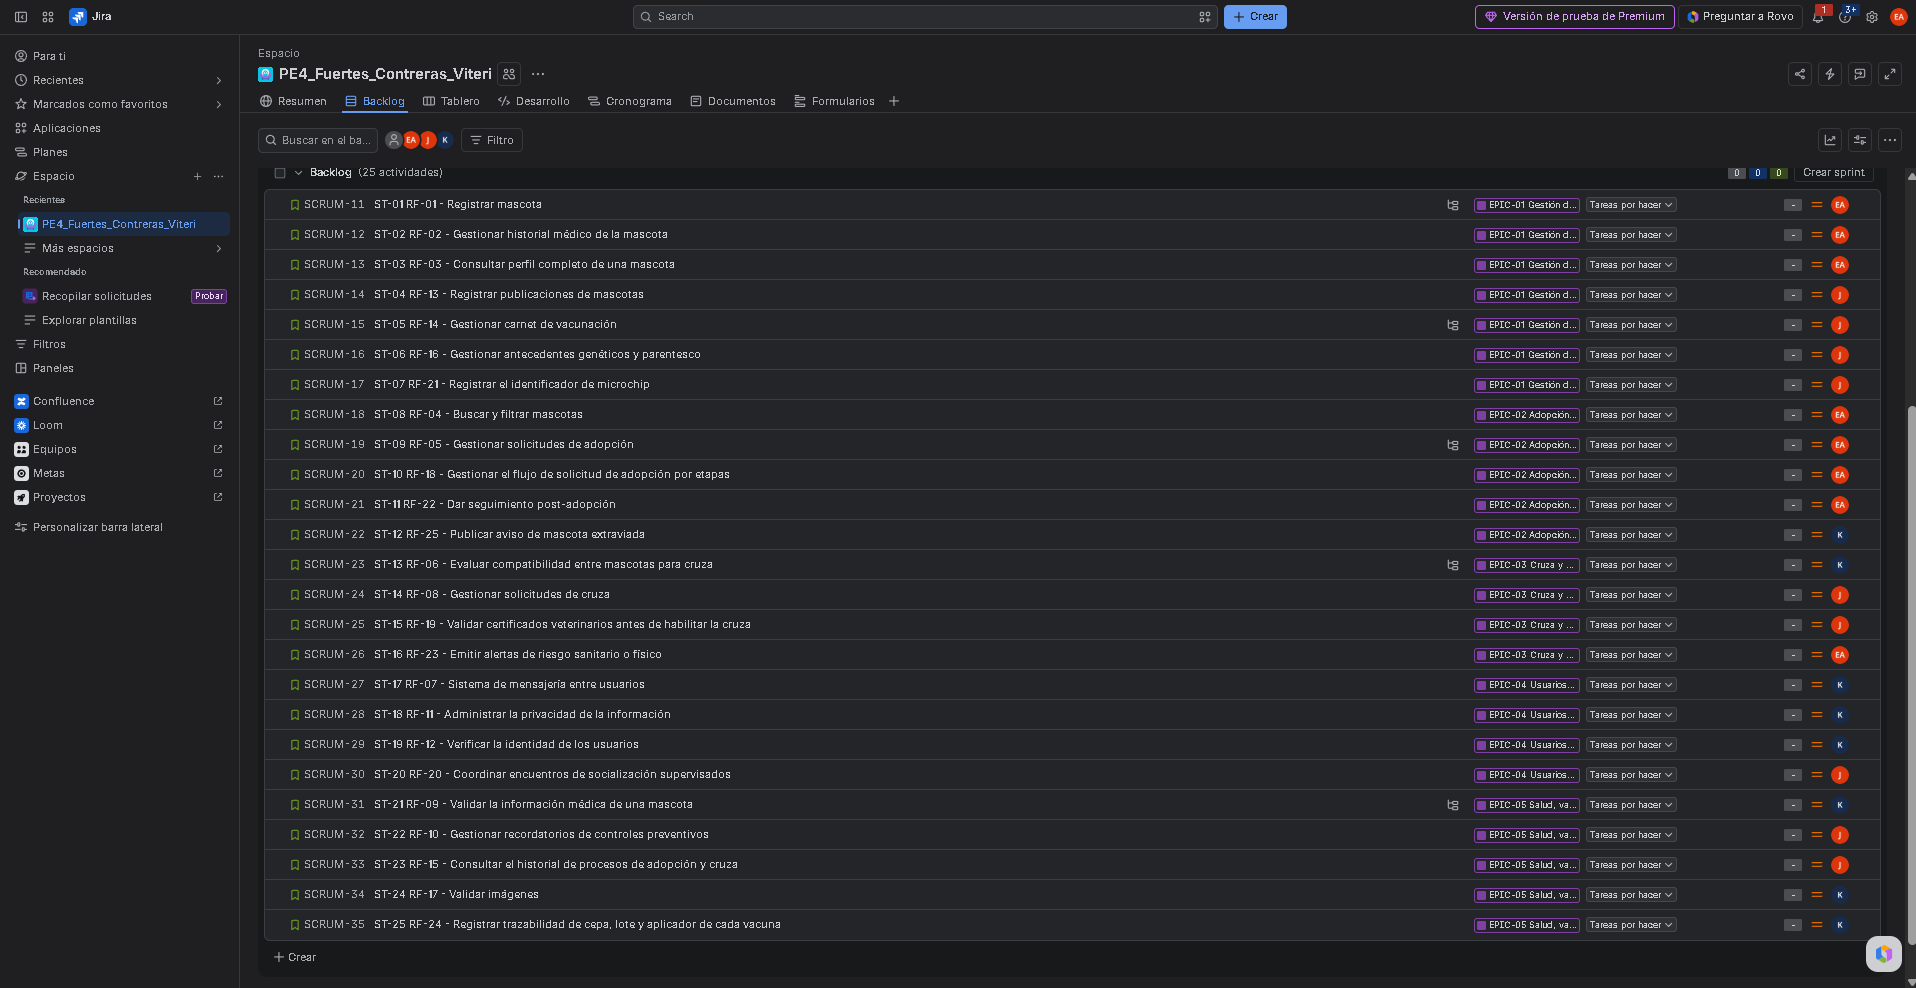
\includegraphics[width=\textwidth]{figuras/tablero_general.png}
		\caption{Vista general del backlog: las 25 Stories con su Epic y su responsable asignado.}
		\label{fig:tablero-general}
	\end{figure}
	
	\subsubsection{Evidencia 2: issues con trazabilidad}
	
	Se seleccionaron tres Stories del tablero para demostrar la trazabilidad entre los requisitos y
	los elementos registrados en la herramienta. En cada captura se comprueba el requisito de origen,
	la prioridad MoSCoW y el estado de verificación en la descripción y en las etiquetas, el Epic
	padre en el campo \emph{Principal}, el criterio de aceptación, la cadena de trazabilidad hasta el
	caso de prueba y las dos sub-tareas asociadas.
	
	\begin{figure}[H]
		\centering
		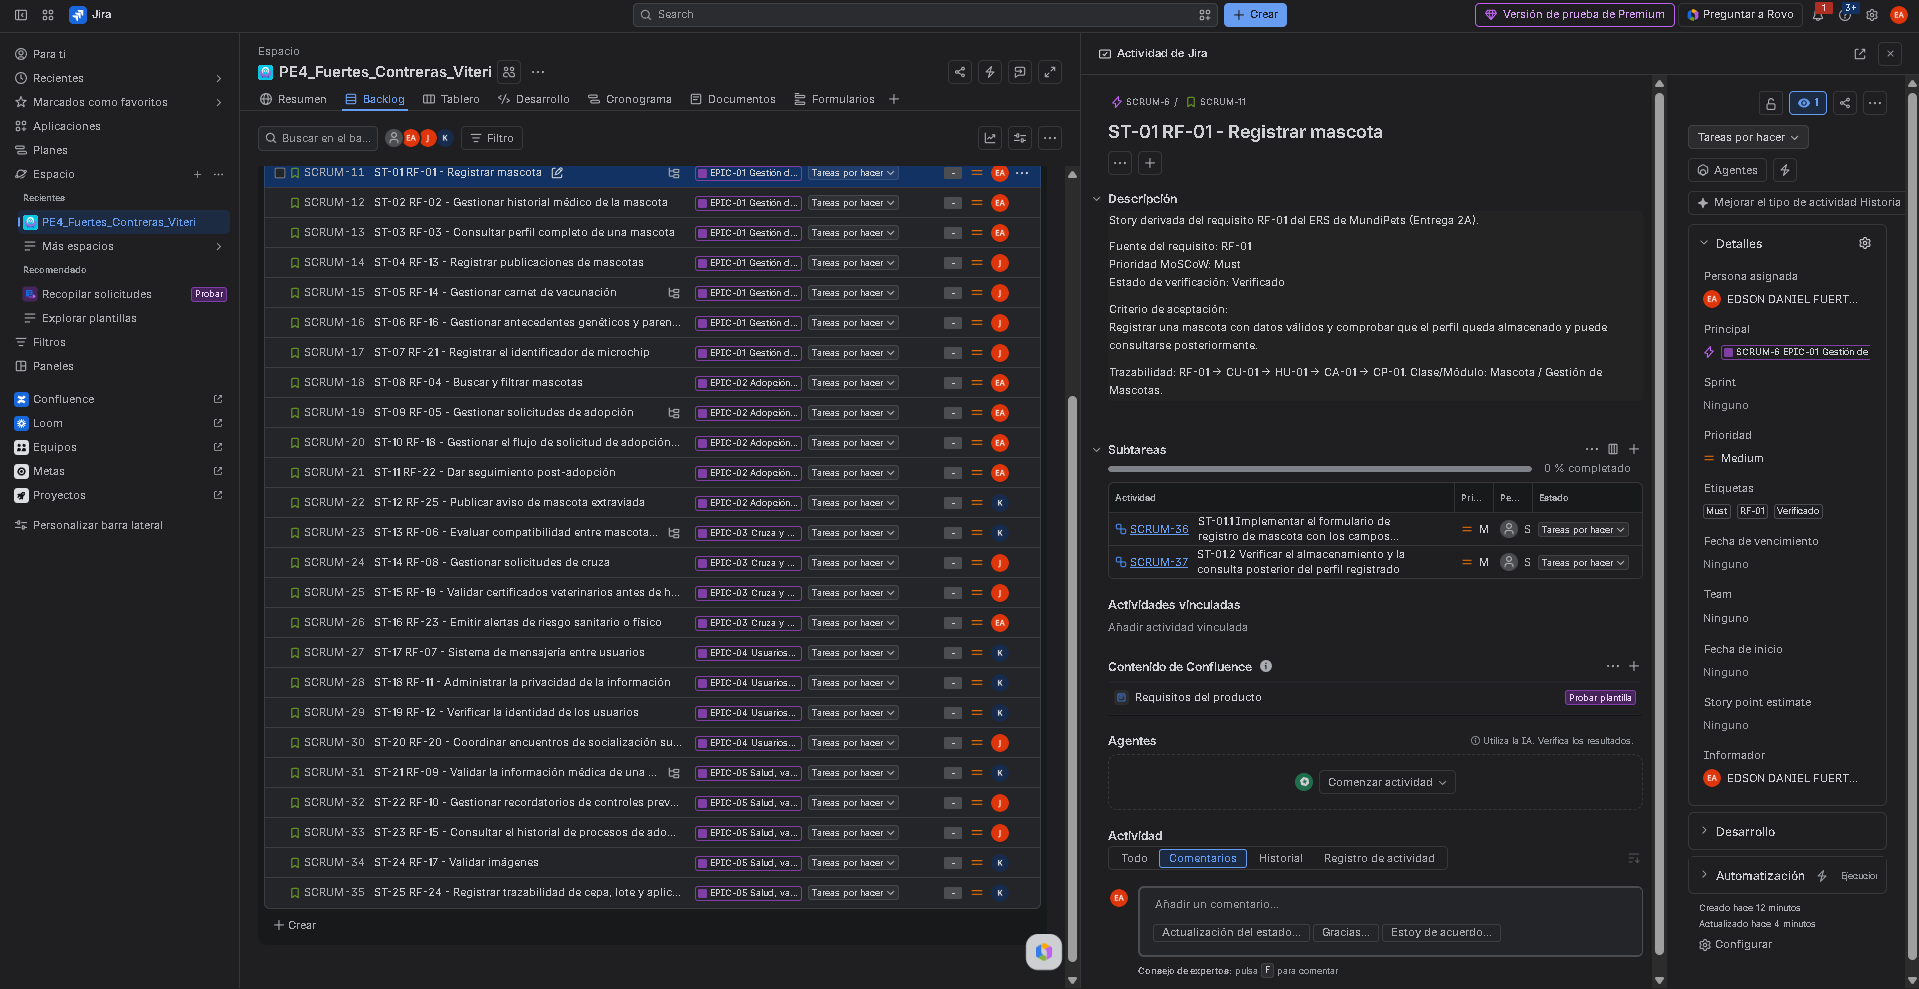
\includegraphics[width=\textwidth]{figuras/tablero_story1.png}
		\caption{SCRUM-11 -- ST-01 (RF-01, Registrar mascota): Epic padre SCRUM-6, etiquetas
			\texttt{Must}, \texttt{RF-01} y \texttt{Verificado}, criterio de aceptación y sub-tareas
			SCRUM-36 y SCRUM-37.}
		\label{fig:story1}
	\end{figure}
	
	\begin{figure}[H]
		\centering
		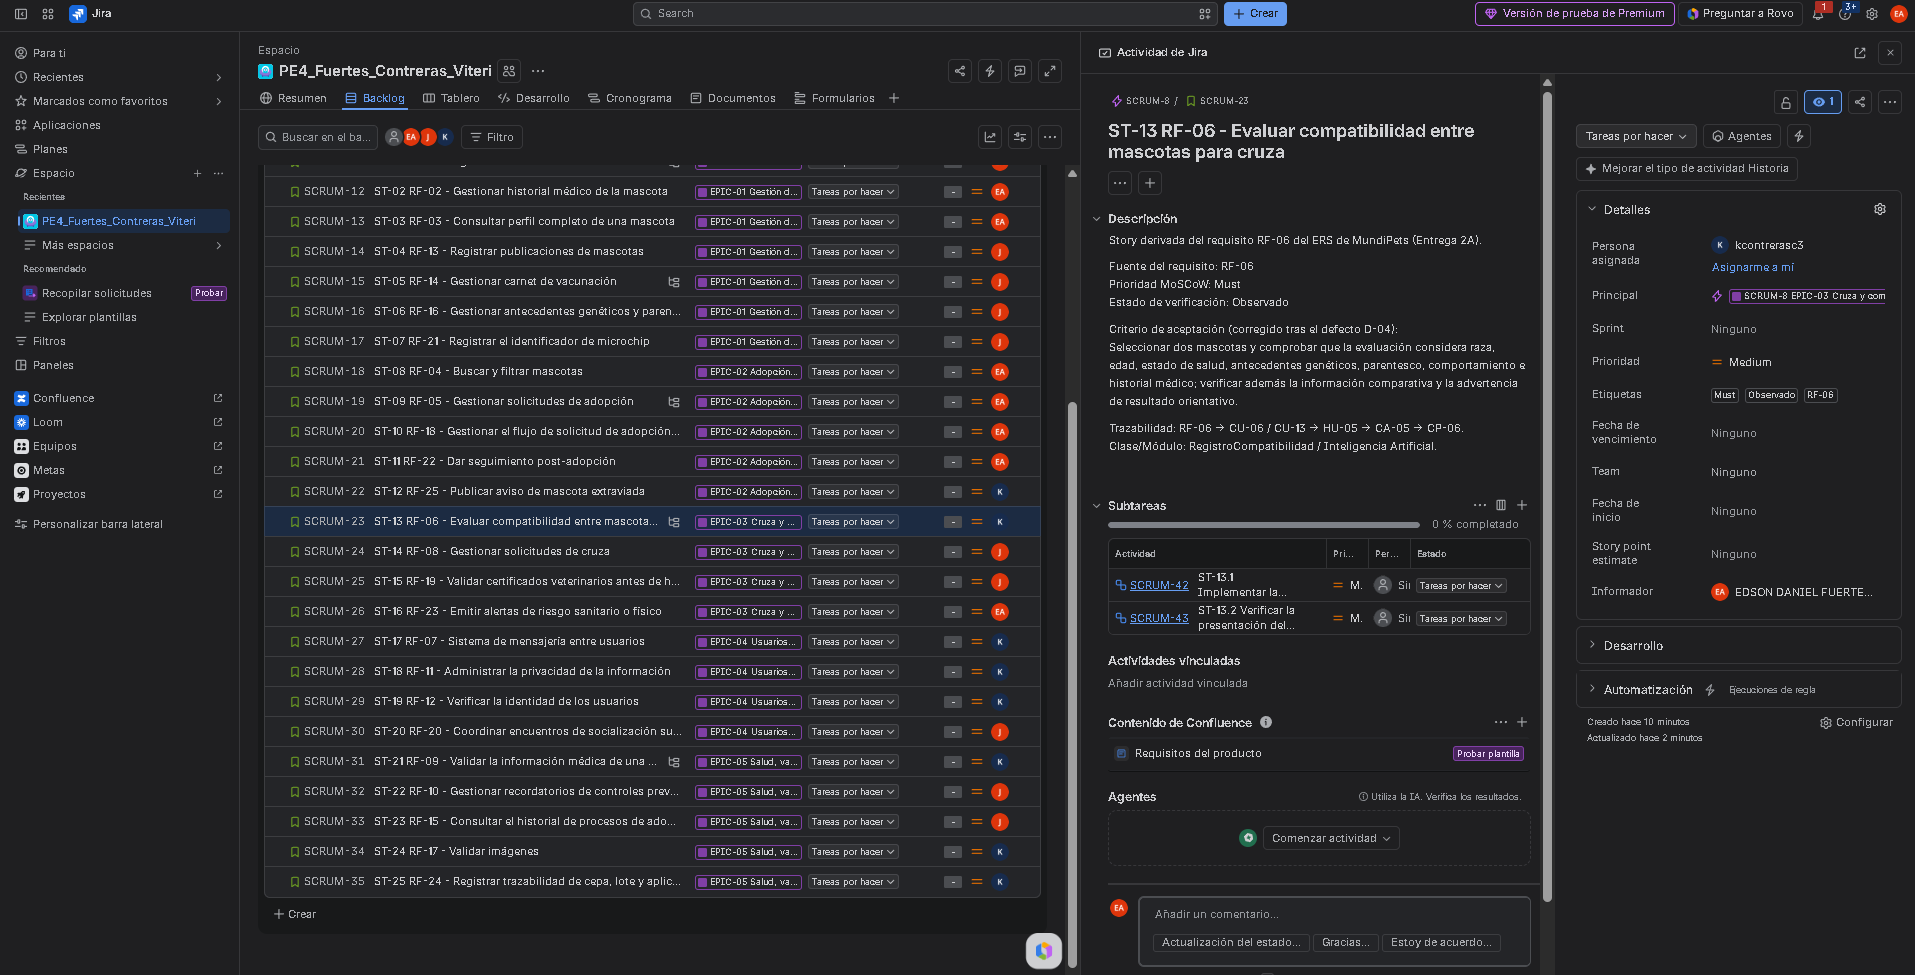
\includegraphics[width=\textwidth]{figuras/tablero_story2.png}
		\caption{SCRUM-23 -- ST-13 (RF-06, Evaluar compatibilidad para cruza): estado
			\texttt{Observado} por el defecto D-04, criterio de aceptación corregido con los siete
			factores y sub-tareas SCRUM-42 y SCRUM-43.}
		\label{fig:story2}
	\end{figure}
	
	\begin{figure}[H]
		\centering
		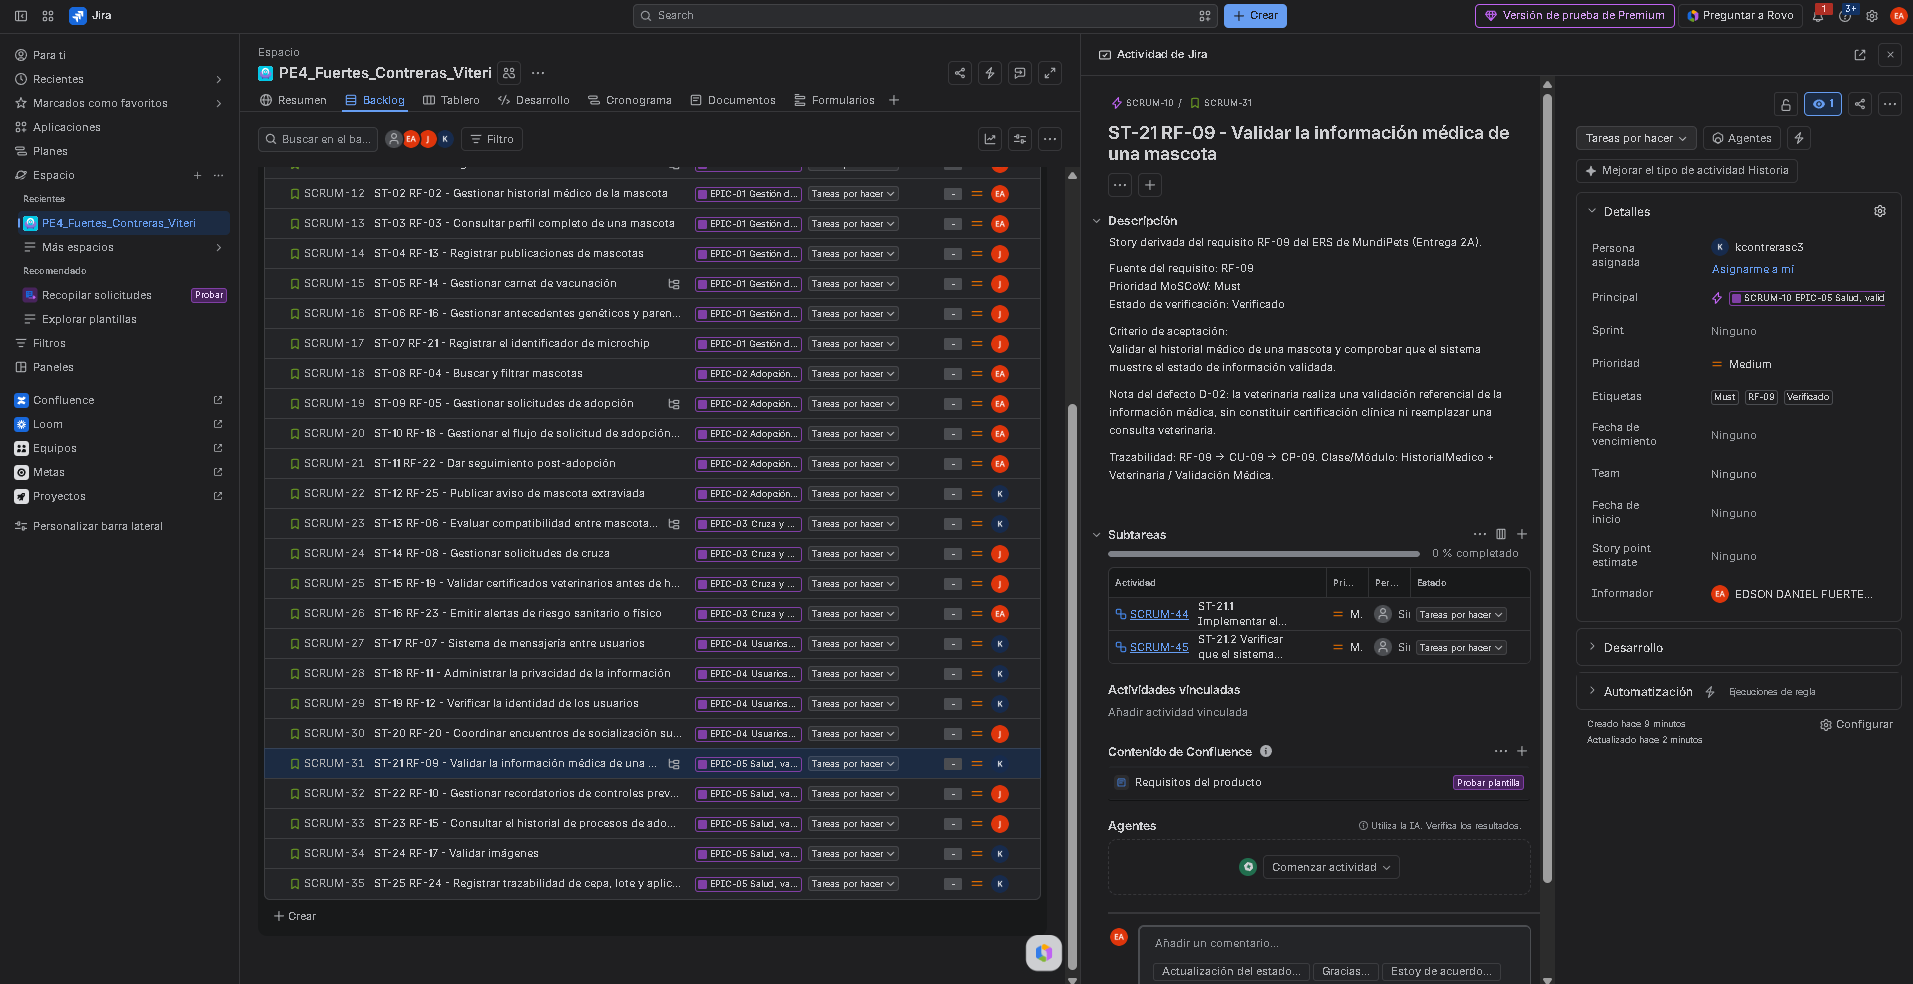
\includegraphics[width=\textwidth]{figuras/tablero_story3.png}
		\caption{SCRUM-31 -- ST-21 (RF-09, Validar la información médica): nota del defecto D-02
			sobre validación referencial, trazabilidad RF-09 $\rightarrow$ CU-09 $\rightarrow$ CP-09 y
			sub-tareas SCRUM-44 y SCRUM-45.}
		\label{fig:story3}
	\end{figure}
	
	Estas evidencias permiten comprobar que las Stories no funcionan únicamente como tareas
	independientes, sino que mantienen una relación con los requisitos documentados en el ERS y con
	los demás artefactos del proyecto.
	
	\subsubsection{Evidencia 3: estadísticas del tablero}
	
	\begin{figure}[H]
		\centering
		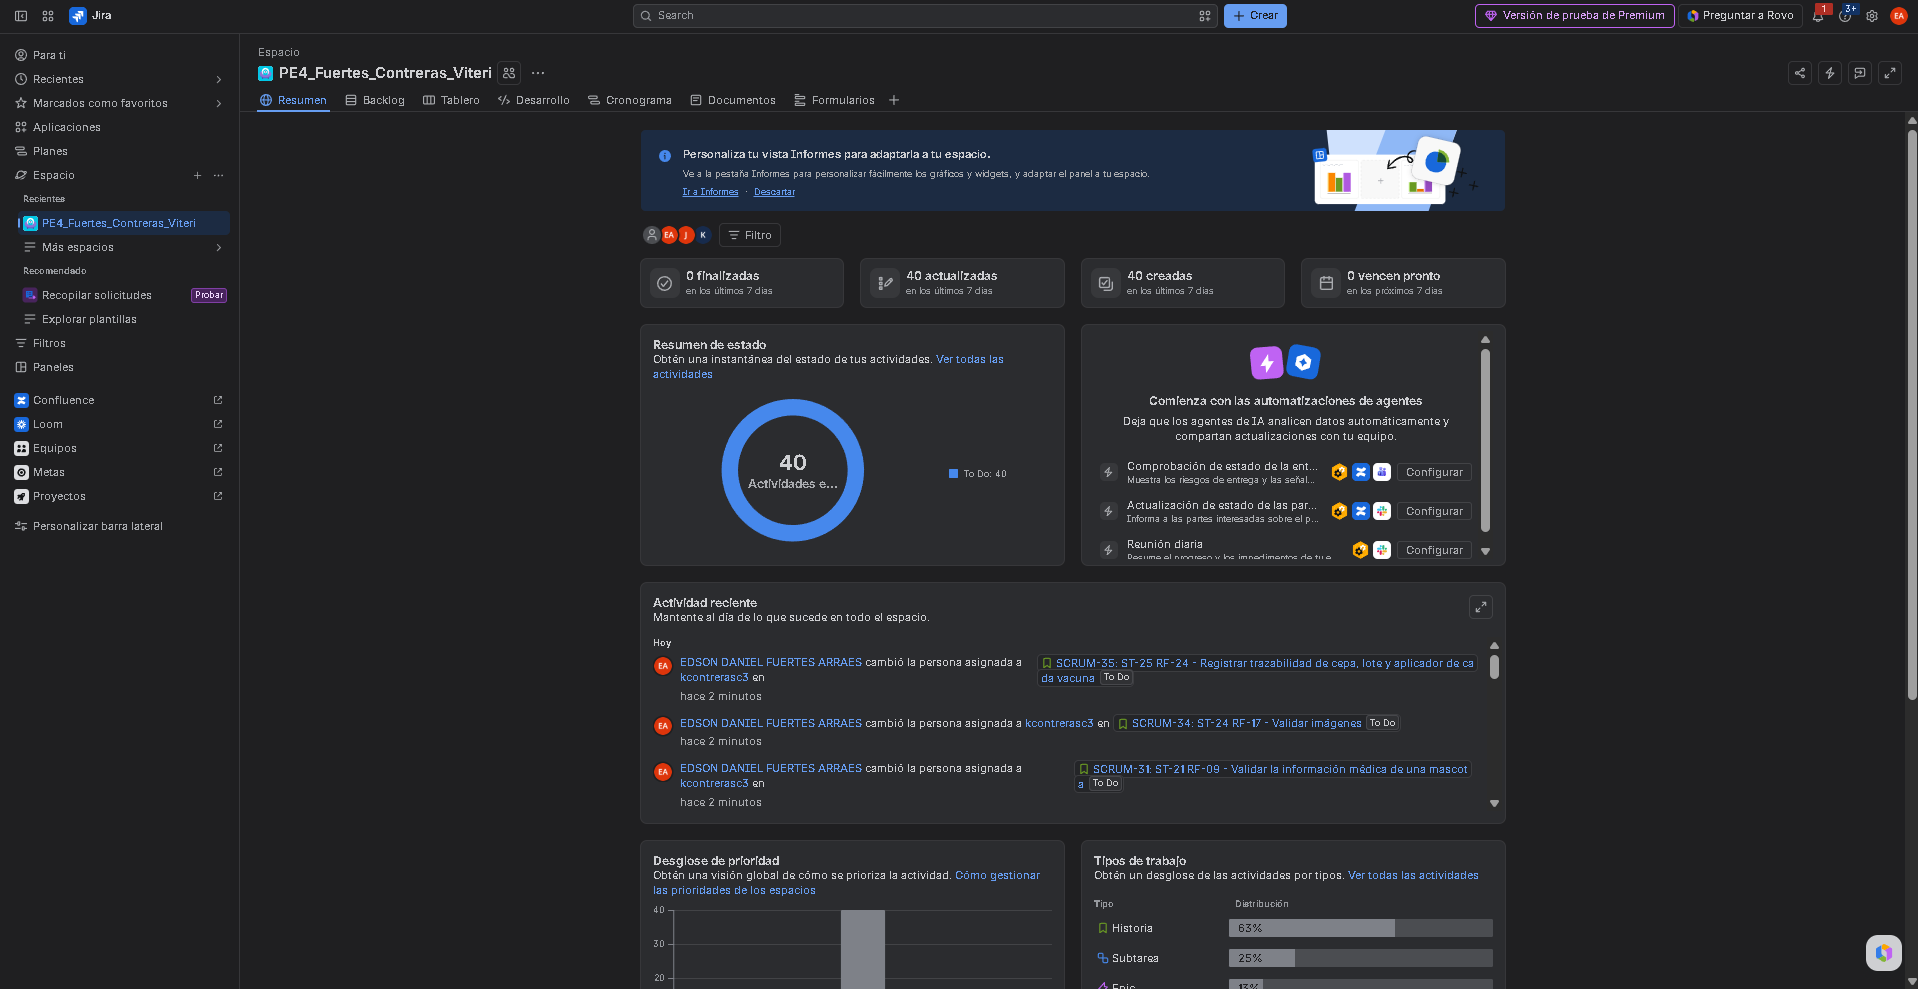
\includegraphics[width=\textwidth]{figuras/tablero_estadisticas.png}
		\caption{Panel de resumen del espacio Jira: 40 actividades creadas y desglose por tipo de
			trabajo.}
		\label{fig:estadisticas}
	\end{figure}
	
	El panel confirma los 40 elementos creados y su desglose por tipo: 63 \% Historia (25 Stories),
	25 \% Subtarea (10 Sub-tasks) y 13 \% Epic (5 Epics), proporciones coherentes con la Tabla
	\ref{tab:tablero-resumen}. El registro de actividad reciente evidencia además la asignación de
	responsables realizada sobre cada elemento. La exportación del backlog en formato CSV se
	referencia en el Anexo D y se encuentra versionada en el repositorio del equipo.
	
	\subsubsection{Coherencia entre las evidencias y el ERS}
	
	Las evidencias recopiladas mantienen correspondencia con la información registrada en el ERS. La
	fuente de cada Story permite identificar el requisito funcional que le dio origen, mientras que
	los criterios de aceptación y las sub-tareas corresponden con los elementos definidos para dicho
	requisito. Además, las Stories cuyo requisito resultó afectado por la inspección o por una RFC
	conservan en su descripción la referencia explícita al defecto o a la solicitud de cambio
	correspondiente (D-02, D-04, D-08, D-09, RFC-01 y RFC-03), lo que permite recorrer la cadena
	completa desde el tablero hasta el registro consolidado de la Sección 3.4 y las decisiones del CCB
	de la Sección \ref{sec:ccb}. De esta manera, las capturas comprueban visualmente que el tablero
	CASE se utilizó como herramienta de apoyo a la gestión y a la trazabilidad de requisitos, y no
	como una simple lista de tareas.
	
	% ═══════════════════════════════════════════════════════════════
	%  SECCIÓN 7 -- LÍNEA BASE CON GIT
	% ═══════════════════════════════════════════════════════════════
	\section{Línea base con Git}
	
	\subsection{Repositorio y estructura}
	
	\subsection{Commits semánticos}
	
	\subsection{Tag anotado de línea base}
	
	\subsection{CHANGELOG.md}
	
	% ═══════════════════════════════════════════════════════════════
	%  SECCIÓN 8 -- COMPARATIVA CASE
	% ═══════════════════════════════════════════════════════════════
	\section{Comparativa de herramientas CASE}
	\label{sec:comparativa}
	
	La comparación usa las seis dimensiones exigidas por la guía. Las afirmaciones sobre las
	herramientas son juicios de adecuación para Ingeniería de Requisitos y se respaldan con fuentes
	oficiales de cada fabricante.
	
	\begin{longtable}{L{1.9cm} L{2.9cm} L{2.9cm} L{2.9cm} L{2.9cm}}
		\caption{Comparativa de herramientas CASE para ingeniería de requisitos}
		\label{tab:case}\\
		\toprule
		\textbf{Criterio} & \textbf{Jira} & \textbf{IBM DOORS Next} & \textbf{Jama Connect} &
		\textbf{ReqView} \\
		\midrule
		\endfirsthead
		\toprule
		\textbf{Criterio} & \textbf{Jira} & \textbf{IBM DOORS Next} & \textbf{Jama Connect} &
		\textbf{ReqView} \\
		\midrule
		\endhead
		\bottomrule
		\endfoot
		Funcionalidades de IR &
		Media. Permite gestionar trabajo mediante issues, campos, prioridades y flujos configurables;
		para una ERS formal requiere convenciones de modelado y enlaces definidos por el equipo
		\cite{atlassian2026}. &
		Muy alta. Está orientada a capturar, trazar, analizar y gestionar cambios en requisitos, con
		visibilidad a lo largo del ciclo de vida \cite{ibmdoors2026}. &
		Muy alta. Permite definir, revisar, trazar y validar requisitos, y relacionarlos con pruebas y
		revisiones formales \cite{jama2026}. &
		Alta. Ofrece gestión estructurada de requisitos, atributos, documentos y trazabilidad
		\emph{end-to-end} \cite{reqview2026}. \\
		\addlinespace
		Trazabilidad &
		Media-alta. Soporta enlaces entre elementos y jerarquías; la cadena requisito--prueba debe
		diseñarse mediante tipos, enlaces y campos del proyecto \cite{atlassian2026}. &
		Alta. Solución web con colaboración, revisiones, historial y trabajo compartido sobre
		requisitos \cite{ibmdoors2026}. &
		Muy alta. Ofrece trazabilidad hacia adelante y hacia atrás, análisis de impacto e informes de
		trazabilidad \cite{jama2026}. &
		Muy alta. Soporta trazabilidad \emph{end-to-end} y gestión de enlaces entre requisitos
		\cite{reqview2026}. \\
		\addlinespace
		Colaboración &
		Alta. Comentarios, responsables, tableros y trabajo web resultan adecuados para un equipo
		académico pequeño \cite{atlassian2026}. &
		Alta. Discusiones y colaboración sobre requisitos en el entorno web \cite{ibmdoors2026}. &
		Muy alta. Revisiones, aprobaciones y colaboración en tiempo real son parte central de la
		plataforma \cite{jama2026}. &
		Media-alta. Colaboración basada en archivos y proyectos y, en planes superiores, trabajo de
		equipo \cite{reqview2026}. \\
		\addlinespace
		Integración con VCS &
		Alta. Integración oficial con GitHub para asociar la actividad de desarrollo con los issues
		\cite{atlassian2026}. &
		Media-alta. Se integra dentro del ecosistema Engineering Lifecycle Management; no usa Git como
		núcleo del repositorio de requisitos \cite{ibmdoors2026}. &
		Media. Dispone de integraciones y API, pero su fortaleza principal es la gestión de requisitos
		y pruebas, no el control de versiones \cite{jama2026}. &
		Alta. Puede gestionar proyectos de requisitos en Git y colaborar con repositorios GitHub,
		GitLab, Bitbucket o Azure DevOps \cite{reqview2026}. \\
		\addlinespace
		Costo &
		Muy favorable para MundiPets: plan gratuito hasta 10 usuarios, suficiente para un equipo de
		tres \cite{atlassian2026}. &
		Desfavorable para presupuesto cero: solución empresarial y comercial \cite{ibmdoors2026}. &
		Desfavorable para presupuesto cero: producto comercial orientado a organizaciones y proyectos
		complejos \cite{jama2026}. &
		Desfavorable para presupuesto cero en funciones completas: los planes PRO y TEAM son de pago
		por usuario \cite{reqview2026}. \\
		\addlinespace
		Curva de aprendizaje &
		Media. Es fácil para tableros; la trazabilidad rigurosa exige configurar tipos, campos y
		enlaces con disciplina. &
		Alta. Es potente, pero requiere aprender módulos, enlaces, \emph{baselines} y
		administración. &
		Media-alta. La interfaz moderna facilita la revisión, pero el modelado de relaciones y
		procesos requiere capacitación. &
		Media. Más directo que las suites empresariales; el uso avanzado de trazabilidad y Git
		requiere práctica. \\
	\end{longtable}
	
	\subsection{Recomendación argumentada para el PFC}
	\label{sec:recomendacion}
	
	Para MundiPets, Jira es la alternativa más conveniente dentro de las cuatro comparadas. La razón
	no es que posea mayor capacidad especializada de Ingeniería de Requisitos que IBM DOORS Next o
	Jama Connect, sino que encaja mejor con las restricciones concretas del PFC: equipo de tres
	personas, presupuesto cero, necesidad de tablero jerárquico y trazabilidad hasta caso de prueba.
	El plan gratuito de Jira Cloud admite hasta 10 usuarios, por lo que cubre al equipo sin costo de
	licencia \cite{atlassian2026}.
	
	IBM DOORS Next y Jama Connect ofrecen una trazabilidad y una gestión de requisitos más
	especializadas, especialmente útiles en entornos empresariales o regulados, pero su costo y
	complejidad no se justifican para una práctica académica de este tamaño \cite{ibmdoors2026,
		jama2026}. ReqView es técnicamente atractivo porque su trazabilidad \emph{end-to-end} y su
	integración con Git se ajustan bien a un ERS versionado; sin embargo, las funciones de gestión
	completas son de pago, lo que contradice el presupuesto cero del escenario \cite{reqview2026}.
	
	La recomendación es utilizar Jira con una configuración disciplinada: Epics por área funcional,
	Stories asociadas a los RF, campos para prioridad MoSCoW y fuente del requisito, enlaces a casos
	de uso y pruebas, y referencias a commits o evidencias cuando existan. La limitación debe quedar
	declarada: Jira no sustituye automáticamente a una herramienta dedicada de \emph{Requirements
		Management}; la calidad de la trazabilidad dependerá de que el equipo mantenga los enlaces de
	forma consistente.
	
	% ═══════════════════════════════════════════════════════════════
	%  SECCIÓN 9 -- IR TRADICIONAL VS ÁGIL
	% ═══════════════════════════════════════════════════════════════
	\section{IR tradicional frente a IR ágil}
	\label{sec:tradicional-agil}
	
	La Ingeniería de Requisitos puede desarrollarse mediante enfoques tradicionales o ágiles. Ambos
	buscan identificar, documentar y gestionar las necesidades del sistema, pero presentan diferencias
	importantes en la manera de gestionar la documentación, los cambios, la participación de los
	stakeholders, las herramientas utilizadas, la velocidad de trabajo y la escalabilidad.
	
	\begin{longtable}{L{2.0cm} L{3.9cm} L{3.9cm} L{3.3cm}}
		\caption{Contraste entre IR tradicional e IR ágil}\label{tab:trad-agil}\\
		\toprule
		\textbf{Dimensión} & \textbf{IR tradicional} & \textbf{IR ágil} &
		\textbf{Contexto donde conviene} \\
		\midrule
		\endfirsthead
		\toprule
		\textbf{Dimensión} & \textbf{IR tradicional} & \textbf{IR ágil} &
		\textbf{Contexto donde conviene} \\
		\midrule
		\endhead
		\bottomrule
		\endfoot
		Documentación &
		Documentación detallada y estructurada antes de avanzar a las siguientes etapas; el ERS es el
		artefacto central que establece la referencia formal \cite{pohl2025}. &
		Documentación más ligera y evolutiva; los requisitos se representan mediante historias de
		usuario, criterios de aceptación y elementos del backlog \cite{cohn2004}. &
		Tradicional cuando existe obligación contractual o de auditoría; ágil cuando el dominio es
		conocido y el cliente está disponible. \\
		\addlinespace
		Gestión del cambio &
		Procesos formales con análisis de impacto, solicitudes de cambio y mecanismos de aprobación
		\cite{pmbok7}. &
		Los cambios se incorporan con mayor frecuencia mediante la actualización y priorización del
		backlog en cada iteración \cite{cohn2004}. &
		Tradicional cuando un cambio arrastra muchos artefactos enlazados; ágil cuando el costo de
		revertir es bajo. \\
		\addlinespace
		Participación de stakeholders &
		Concentrada en actividades específicas de levantamiento, validación y aprobación
		\cite{wiegers2013}. &
		Participación frecuente para obtener retroalimentación y validar los incrementos
		desarrollados. &
		Tradicional con stakeholders dispersos o de disponibilidad limitada; ágil con un
		\emph{product owner} accesible. \\
		\addlinespace
		Herramientas &
		Documentos formales, matrices de trazabilidad, herramientas de modelado y sistemas de gestión
		documental. &
		Herramientas de backlog, tableros, historias de usuario, seguimiento de tareas y colaboración
		continua. &
		Tradicional cuando se exige trazabilidad auditable; ágil cuando prima la visibilidad del flujo
		de trabajo. \\
		\addlinespace
		Velocidad &
		El levantamiento y la documentación detallada requieren más tiempo al inicio, pero
		proporcionan una referencia estable para las etapas posteriores. &
		Permite obtener resultados y retroalimentación de manera incremental, reduciendo el tiempo
		entre la definición del requisito y la validación de la funcionalidad. &
		Tradicional cuando el costo del error es alto; ágil cuando el requisito debe validarse con
		usuarios reales antes de consolidarse. \\
		\addlinespace
		Escalabilidad &
		Apropiado para proyectos grandes o regulados donde se requiere alto nivel de documentación,
		control y trazabilidad formal. &
		Escala mediante equipos, iteraciones y mecanismos de coordinación, aunque los proyectos
		grandes exigen disciplina adicional para mantener la trazabilidad entre equipos
		\cite{smart2014}. &
		Tradicional en sistemas con múltiples subsistemas interdependientes; ágil en equipos pequeños
		y autónomos como el de esta práctica. \\
	\end{longtable}
	
	\subsection{Discusión contextual}
	
	En el caso de MundiPets, ambos enfoques presentan ventajas. El enfoque tradicional resulta útil
	para establecer una especificación formal mediante el ERS, mantener una matriz de trazabilidad,
	controlar versiones y gestionar cambios mediante RFC y el Change Control Board. Estas prácticas
	permiten mantener un registro verificable de las decisiones y de las relaciones entre los
	requisitos y los demás artefactos del proyecto.
	
	Por otra parte, el enfoque ágil resulta conveniente para la evolución de las funcionalidades,
	debido a que permite organizar los requisitos mediante historias de usuario, criterios de
	aceptación y un backlog que puede actualizarse conforme cambien las necesidades del proyecto. El
	tablero CASE construido en la Sección 6 representa precisamente una forma de organizar los
	requisitos más cercana a un flujo de trabajo ágil.
	
	La experiencia concreta de esta práctica aporta un argumento a favor de combinar ambos. Los dos
	defectos críticos del ERS, D-10 y D-11, son contradicciones entre RF-25 y RNF-16 situadas en
	secciones distintas del documento: son exactamente el tipo de defecto que un backlog de historias
	independientes no habría expuesto, porque ninguna historia individual contiene ambas condiciones a
	la vez. Se detectaron gracias a una lectura documental transversal. En sentido inverso, la
	volatilidad del 22 \% calculada en la Sección 2.3 muestra que fijar toda la especificación por
	adelantado tampoco garantizó estabilidad: casi uno de cada cuatro elementos requirió modificación.
	
	\subsubsection{Enfoque recomendado}
	
	Para MundiPets se recomienda un \textbf{enfoque híbrido}. El enfoque tradicional debe utilizarse
	para aquellos elementos que requieren mayor formalidad y control: el ERS, la línea base, la matriz
	de trazabilidad, las solicitudes RFC y las decisiones del CCB. Esto permite mantener una
	referencia documental y controlar los cambios que puedan afectar a varios artefactos a la vez.
	
	El enfoque ágil debe utilizarse para gestionar el trabajo cotidiano mediante historias de usuario,
	criterios de aceptación en Gherkin, prioridades MoSCoW y el tablero CASE. De esta manera el equipo
	organiza y prioriza el trabajo de forma incremental sin perder la trazabilidad establecida en el
	ERS.
	
	El proyecto es un caso particularmente favorable para esta combinación porque el ERS es fuertemente
	documental pero ya incorpora historias de usuario (HU-01 a HU-15) y criterios de aceptación en
	Gherkin. El enfoque híbrido no exige, por tanto, reconstruir artefactos: exige mantener
	sincronizadas dos representaciones que el equipo ya produce.
	
	% ═══════════════════════════════════════════════════════════════
	%  SECCIÓN 10 -- CONCLUSIONES
	% ═══════════════════════════════════════════════════════════════
	\section{Conclusiones críticas}
	
	\subsection*{C1 -- Validación e inspección Fagan}
	
	La inspección aplicada al ERS de MundiPets evidencia que la validación formal aporta valor cuando
	se cruza un requisito con el resto de artefactos y no se revisa de manera aislada. El registro
	consolidado del Inspector 2 documenta 15 defectos: los de mayor impacto aparecen en la privacidad
	de RF-25 frente a RNF-16, en la coherencia del bloque de IA y en los enlaces de trazabilidad.
	Además, la preparación individual de Kevin Contreras identifica seis hallazgos previos desde las
	perspectivas de ambigüedad, completitud y consistencia, cumpliendo el mínimo exigido para llegar a
	la reunión con evidencia preparada. La principal lección es que un ERS extenso puede contener
	requisitos individualmente detallados y, aun así, mantener contradicciones entre secciones, casos
	de uso y matriz.
	
	\subsection*{C2 -- Métricas y calidad del ERS}
	
	La distribución de los 15 hallazgos muestra que el problema dominante no es la falta total de
	requisitos, sino la coherencia entre artefactos. Se registran 7 defectos de consistencia, 2 de
	ambigüedad, 2 de completitud y 4 de trazabilidad; además, 14 de 15 (93,3 \%) fueron clasificados
	como críticos o mayores. Esto indica que la prioridad de mejora del ERS debe concentrarse en
	sincronizar requisitos, conflictos, UML y matriz cuando se incorporan nuevas funciones. Los casos
	RF-24 y RF-25 demuestran el efecto: un dato omitido (el ``lote'') o una condición de privacidad
	contradictoria pueden mantenerse en varias secciones si no existe una revisión transversal antes
	de establecer la línea base.
	
	\subsection*{C3 -- Gestión del cambio y control de configuración}
	
	La gestión de requisitos y el control de configuración resultaron determinantes para mantener la
	coherencia del proyecto ante las modificaciones. El uso de líneas base, versionado, trazabilidad y
	solicitudes de cambio permitió identificar qué requisitos quedaban afectados y evaluar las
	consecuencias antes de incorporar cada modificación al ERS. El dato que lo demuestra es el
	recorrido de la RFC-03: partiendo de un único requisito, RF-25, el análisis por matriz reveló
	impacto sobre RF-11, RNF-16, RD-04 y la fila TR-38, cuatro elementos que una estimación
	``a ojo'' no habría identificado. El proceso RFC y la participación del Change Control Board
	proporcionaron el mecanismo formal para analizar y decidir sobre los tres cambios, con un costo
	comprometido de 14 horas-persona y una volatilidad resultante del 22 \% en el paso de v1.0 a v1.1.
	
	\subsection*{C4 -- Trazabilidad y herramienta CASE}
	
	La construcción del tablero CASE evidenció que la trazabilidad no se obtiene por el hecho de usar
	una herramienta, sino por la disciplina con que se mantienen los enlaces. Los 25 RF del ERS se
	representaron como Stories dentro de cinco Epics, con los campos Prioridad MoSCoW, Fuente del
	requisito y Estado de verificación, y la matriz bidireccional de 15 filas extendió la cadena del
	ERS hasta el caso de prueba, tramo que el documento original no cubría. El hallazgo más útil fue
	el inverso: al proyectar la matriz aparecieron diez RF con tramos incompletos o incorrectos hacia
	adelante, entre ellos cuatro enlaces semánticamente equivocados (TR-10, TR-11, TR-33 y TR-38) que
	apuntaban a casos de uso de otra finalidad. Un requisito con un enlace incorrecto resulta más
	peligroso que uno sin enlace, porque aparenta estar trazado y no lo está.
	
	\subsection*{C5 -- Línea base y contraste tradicional/ágil}
	
	% ═══════════════════════════════════════════════════════════════
	%  SECCIÓN 11 -- DISTRIBUCIÓN DEL TRABAJO
	% ═══════════════════════════════════════════════════════════════
	\section{Distribución del trabajo}
	
	\begin{table}[H]
		\centering
		\caption{Aportes por integrante}
		\label{tab:distribucion}
		\begin{tabular}{L{3.8cm} L{6.0cm} L{1.6cm} L{1.6cm}}
			\toprule
			\textbf{Integrante} & \textbf{Secciones y artefactos} & \textbf{Horas} &
			\textbf{Commits} \\
			\midrule
			Fuertes Arraes Edson Daniel &
			Coordinación, carátula, resumen y objetivos (1), planificación y acta de inspección
			(3.1, 3.3), versión resultante del ERS (5.5), línea base con Git (7), conclusión C5,
			distribución (11), Anexos E y F, integración y compilación & & \\
			\addlinespace
			Contreras Chávez Kevin Germán &
			Fundamento 2.1, 2.2 y 2.5; preparación individual (3.2); registro de defectos (3.4);
			correcciones (4); RFC-01 y RFC-03; matriz de trazabilidad y huérfanos (6.3, 6.4);
			comparativa CASE (8); conclusiones C1 y C2; Anexos A (su copia), B y C & & \\
			\addlinespace
			Viteri García Jonathan Enrique &
			Fundamento 2.3 y 2.4; preparación individual (3.2); métricas y gráficos (3.5);
			RFC-02 y redacción del acta del CCB (5.4); tablero, campos y evidencias
			(6.1, 6.2, 6.5); IR tradicional frente a ágil (9); conclusiones C3 y C4;
			Anexos A (su copia) y D & & \\
			\bottomrule
		\end{tabular}
	\end{table}
	
	% ═══════════════════════════════════════════════════════════════
	%  REFERENCIAS
	% ═══════════════════════════════════════════════════════════════
	\printbibliography[title={Referencias}]
	
	% ═══════════════════════════════════════════════════════════════
	%  ANEXOS
	% ═══════════════════════════════════════════════════════════════
	\appendix
	\section*{Anexos}
	\addcontentsline{toc}{section}{Anexos}
	
	\subsection*{Anexo A -- Listas de verificación de inspección}
	
	\subsubsection*{Anexo A.1 -- Inspector 1: Viteri García Jonathan Enrique}
	
	Checklist individual firmado y fechado, guardado con marca temporal verificable antes de la
	reunión. La perspectiva asignada fue verificabilidad, trazabilidad y factibilidad, aplicada sobre
	los 16 RNF de la Sección 3 del ERS.
	
	\begin{longtable}{L{1.6cm} L{3.3cm} L{1.4cm} C{1.0cm} L{2.85cm} L{2.65cm}}
		\caption{Anexo A.1 -- Lista de verificación de inspección del Inspector 1}
		\label{tab:anexoA-jonathan}\\
		\toprule
		\textbf{Propiedad} & \textbf{Pregunta de verificación} & \textbf{Req. revisado} &
		\textbf{Cumple} & \textbf{Evidencia} & \textbf{Observación} \\
		\midrule
		\endfirsthead
		\toprule
		\textbf{Propiedad} & \textbf{Pregunta de verificación} & \textbf{Req. revisado} &
		\textbf{Cumple} & \textbf{Evidencia} & \textbf{Observación} \\
		\midrule
		\endhead
		\bottomrule
		\endfoot
		Verificabilidad & ¿El umbral declarado puede medirse con un procedimiento definido? &
		RNF-06 / RNF-07 & No &
		``Conjunto representativo de casos'' y ``tipo de fotografía esperado'' sin definir. &
		Fijar tamaño de muestra y tipos válidos; J-01 y J-02 / D-16 y D-17. \\
		\addlinespace
		Trazabilidad & ¿Los elementos necesarios para verificar el RNF están enlazados en la matriz? &
		RNF-13 / RNF-14 & No &
		Solo se enlaza el RF; faltan evidencia, medición y encuesta. &
		Añadir enlaces explícitos; J-04 y J-05 / D-19 y D-20. \\
		\addlinespace
		Factibilidad & ¿Existen infraestructura y evidencia suficientes para cumplir y comprobar el
		requisito? & RNF-03 / RNF-06 & No &
		No se declara entorno de carga ni conjunto evaluado por veterinarios. &
		Origen de la RFC-02; J-06 y J-07 / D-21 y D-22. \\
		\addlinespace
		Ambigüedad & ¿Los términos cuantitativos del RNF admiten una única lectura? & RNF-12 & No &
		``Degradación significativa'' carece de umbral propio. &
		Cuantificar o eliminar la cláusula; J-08 / D-23. \\
		\addlinespace
		Completitud & ¿El RNF declara todas las condiciones de entorno necesarias para la prueba? &
		RNF-11 & No & No fija versiones de navegador ni resoluciones concretas. &
		Enumerar versiones y resoluciones; J-03 / D-18. \\
		\addlinespace
		Consistencia & ¿Los umbrales de los RNF de rendimiento son mutuamente coherentes? &
		RNF-03 / RNF-12 & Sí &
		P95 $\leq$ 2 s con 100 usuarios y P95 $\leq$ 3 s con 300 usuarios son compatibles entre sí. &
		Mantener la coherencia tras aplicar la RFC-02. \\
	\end{longtable}
	
	\noindent\textbf{Fecha y hora:} 08/08/2026 -- 18:40\\[10pt]
	\textbf{Firma del inspector:} \rule{6cm}{0.4pt}\\[6pt]
	\textbf{Nombre del inspector:} Viteri García Jonathan Enrique
	
	\subsubsection*{Anexo A.2 -- Inspector 2: Contreras Chávez Kevin Germán}
	
	Checklist individual firmado y fechado, guardado con marca temporal verificable antes de la
	reunión. La tabla combina las seis propiedades exigidas por la guía con evidencia tomada del ERS
	Entrega 2A.
	
	\begin{longtable}{L{1.6cm} L{3.3cm} L{1.4cm} C{1.0cm} L{2.85cm} L{2.65cm}}
		\caption{Anexo A.1 -- Lista de verificación de inspección del Inspector 2}
		\label{tab:anexoA-kevin}\\
		\toprule
		\textbf{Propiedad} & \textbf{Pregunta de verificación} & \textbf{Req. revisado} &
		\textbf{Cumple} & \textbf{Evidencia} & \textbf{Observación} \\
		\midrule
		\endfirsthead
		\toprule
		\textbf{Propiedad} & \textbf{Pregunta de verificación} & \textbf{Req. revisado} &
		\textbf{Cumple} & \textbf{Evidencia} & \textbf{Observación} \\
		\midrule
		\endhead
		\bottomrule
		\endfoot
		Ambigüedad & ¿Los términos del requisito admiten una interpretación única? & RF-12 & No &
		``Información/\allowbreak documentación requerida'' sin mecanismo cerrado. &
		Precisar el mecanismo de verificación; se registra P-02 / D-03. \\
		\addlinespace
		Completitud & ¿El requisito contiene todos los datos y condiciones necesarios para su
		propósito? & RF-24 & No & El título incluye el lote; descripción, entradas y criterio no. &
		Agregar el lote en los tres campos; P-06 / D-09. \\
		\addlinespace
		Consistencia & ¿El requisito es compatible con otros requisitos y reglas del ERS? &
		RF-25 / RNF-16 & No & RF-25 hace público el contacto; RNF-16 lo oculta por defecto. &
		Corregir exposición pública y ubicación; D-10 y D-11. \\
		\addlinespace
		Verificabilidad & ¿El resultado esperado puede comprobarse objetivamente con el criterio
		definido? & RF-06 & No &
		El criterio no comprueba los siete factores exigidos por la descripción. &
		Ampliar el criterio de verificación; P-03 / D-04. \\
		\addlinespace
		Trazabilidad & ¿Los enlaces hacia casos de uso corresponden semánticamente al requisito? &
		RF-11 & No & TR-11 enlaza RF-11 con CU-06 aunque CU-12 es privacidad. &
		Corregir TR-11 a CU-12; D-13. \\
		\addlinespace
		Factibilidad & ¿La solución prevista tiene dependencias y riesgos identificados y acotados? &
		RF-10 / RD-08 & Sí &
		El ERS identifica WhatsApp Business API y canal de respaldo in-app. &
		Mantener la dependencia documentada y probar integración y \emph{fallback}. \\
	\end{longtable}
	
	\noindent\textbf{Fecha y hora:} 08/08/2026 -- 21:01\\[10pt]
	\textbf{Firma del inspector:} \rule{6cm}{0.4pt}\\[6pt]
	\textbf{Nombre del inspector:} Contreras Chávez Kevin Germán
	
	\subsection*{Anexo B -- Registro de defectos}
	
	\begin{sloppypar}
		El registro completo corresponde a la Tabla \ref{tab:defectos} de la Sección 3.4. El archivo
		\texttt{02\_Inspeccion/AnexoB\_registro\_defectos.xlsx} del repositorio contiene
		exactamente las mismas 23 filas, sin cambiar identificadores ni severidades, e incorpora una
		columna adicional que identifica al inspector que aportó cada hallazgo.
	\end{sloppypar}
	
	\begin{figure}[H]
		\centering
		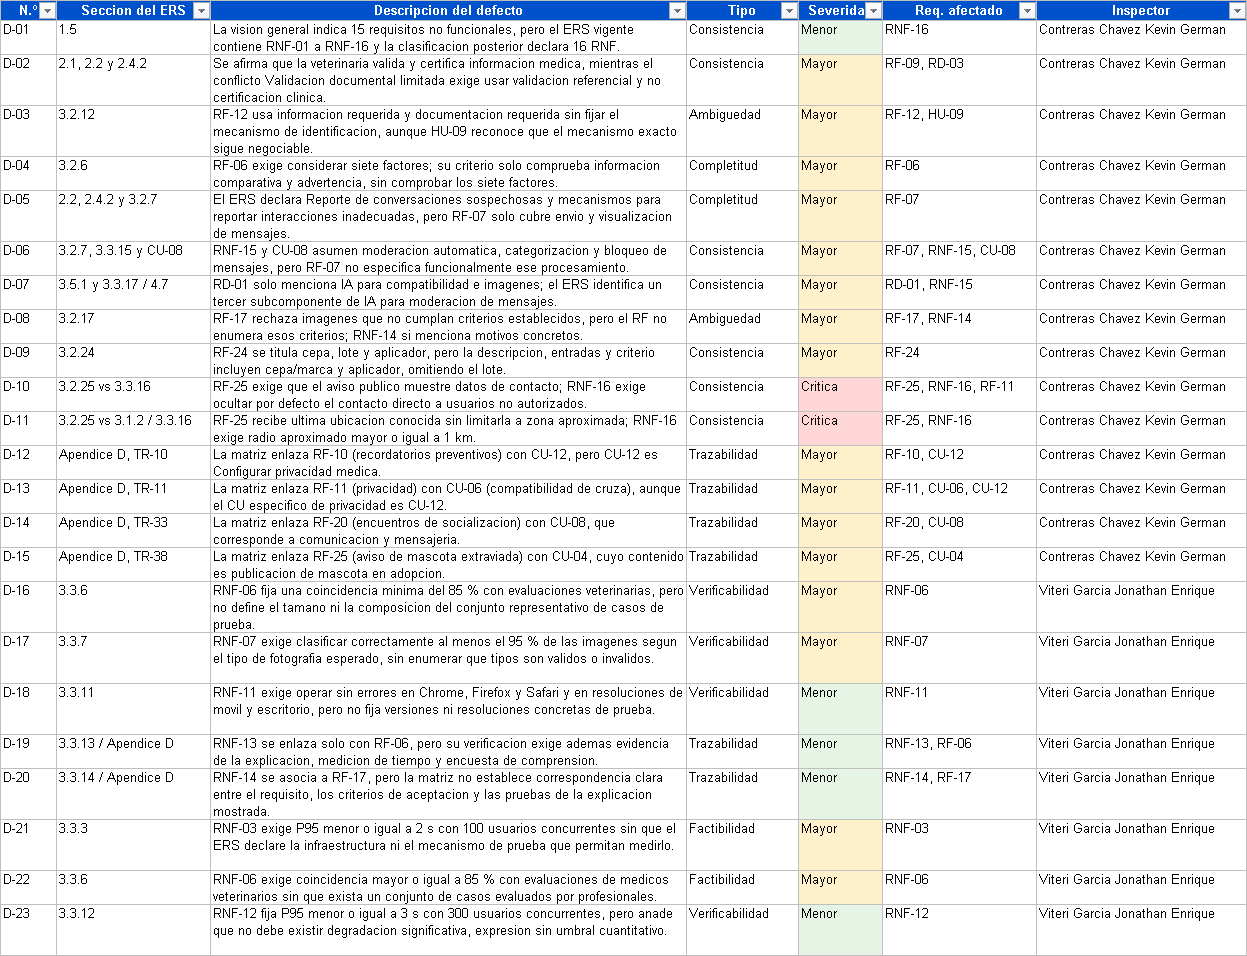
\includegraphics[width=\textwidth]{figuras/anexoB_registro.png}
		\caption{Registro consolidado de los 23 defectos en el archivo del Anexo B, con el
			coloreado por severidad y la atribución por inspector.}
		\label{fig:anexoB-registro}
	\end{figure}
	
	Las cinco métricas de la Sección 3.5 no se transcriben al archivo como valores fijos: se
	calculan mediante fórmulas \texttt{COUNTIF} y \texttt{COUNTA} sobre la hoja de registro, de modo
	que cualquier modificación del conjunto de defectos actualiza automáticamente la densidad, las dos
	distribuciones, las tasas de detección y el esfuerzo. Los únicos datos introducidos manualmente
	son las páginas inspeccionadas y las horas de preparación de cada inspector, resaltados en azul.
	
	\begin{figure}[H]
		\centering
		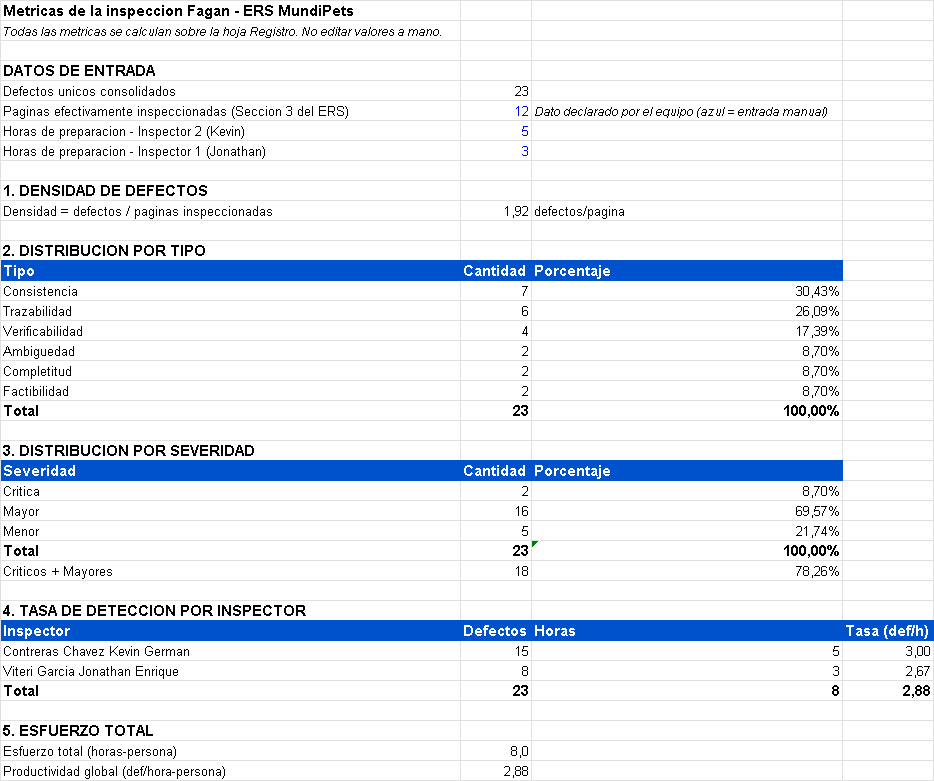
\includegraphics[width=0.95\textwidth]{figuras/anexoB_metricas.png}
		\caption{Hoja de métricas del Anexo B: las cinco métricas calculadas por fórmula sobre el
			registro de defectos.}
		\label{fig:anexoB-metricas}
	\end{figure}
	
	\subsection*{Anexo C -- Formularios RFC y acta del CCB}
	
	Los formularios completos se transcriben en las Tablas \ref{tab:rfc01} y \ref{tab:rfc03} de la
	Sección \ref{sec:ccb}. Los PDF correspondientes se encuentran versionados en
	\texttt{03\_CCB/RFC-01.pdf} y \texttt{03\_CCB/RFC-03.pdf}, y coinciden con lo transcrito en el
	informe.
	
	\subsection*{Anexo D -- Exportación CSV del backlog}
	
	\begin{sloppypar}
		El backlog completo del tablero CASE se exportó en formato CSV y se encuentra versionado en el
		repositorio como \texttt{04\_Trazabilidad/backlog\_export.csv}. El archivo contiene una fila
		por elemento del tablero (5 Epics, 25 Stories y 10 Sub-tasks) con las columnas de clave, tipo,
		resumen, Fuente del requisito, Prioridad MoSCoW y Estado de verificación, de modo que la
		correspondencia con la Tabla \ref{tab:tablero} y con la matriz de la Sección 6.3 puede
		comprobarse directamente sobre el archivo.
	\end{sloppypar}
	
	\begin{figure}[H]
		\centering
		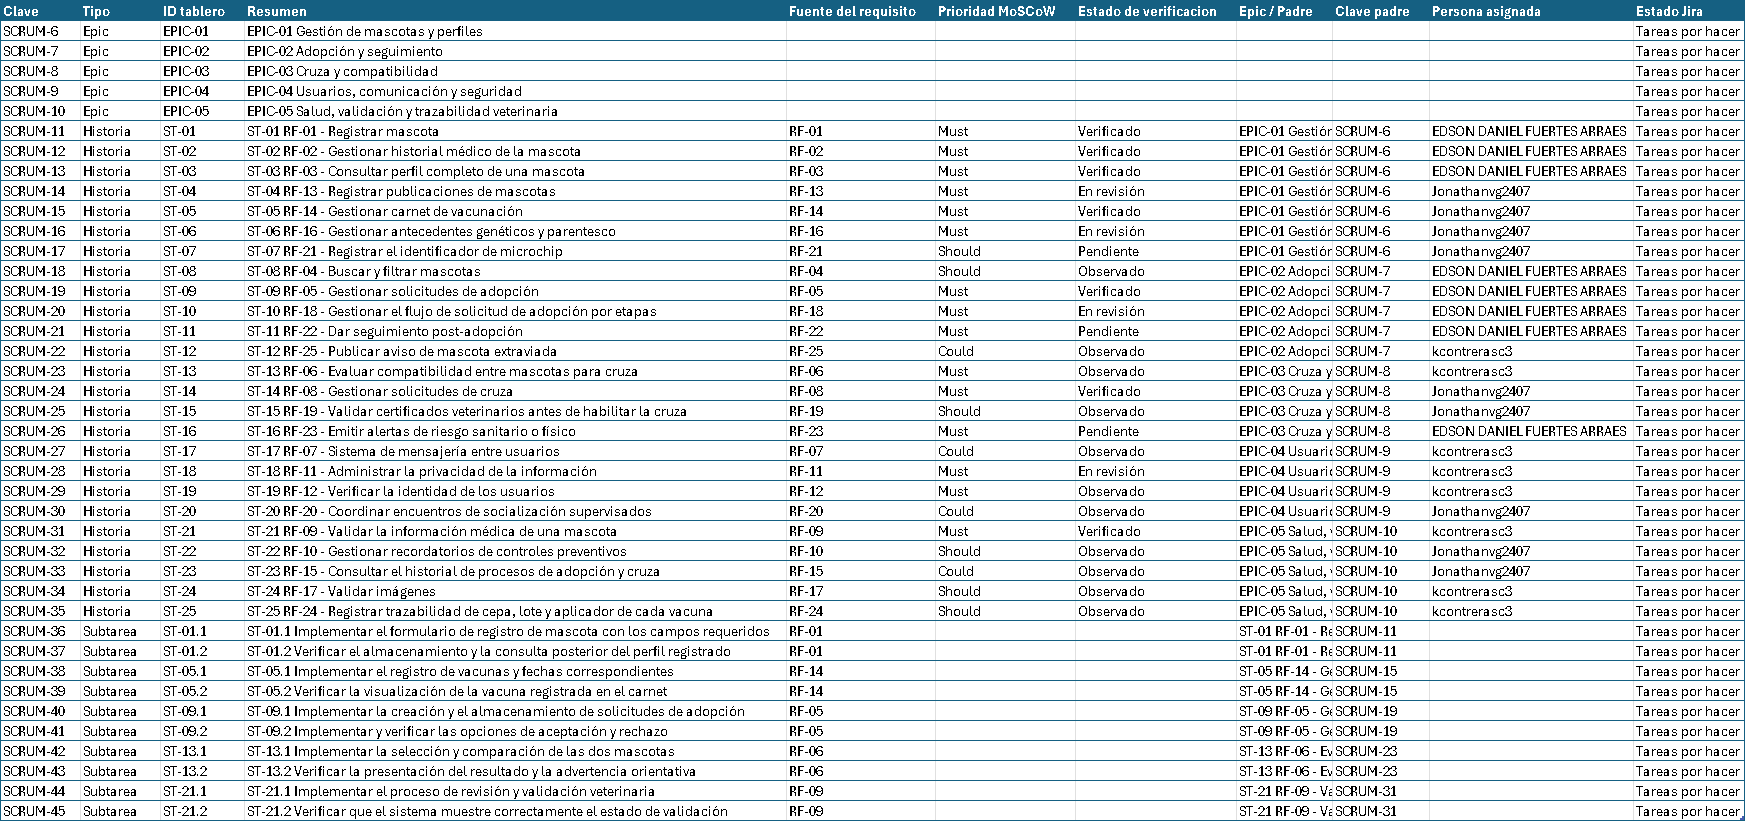
\includegraphics[width=0.88\textwidth]{figuras/backlog_csv.png}
		\caption{Exportación del backlog del tablero CASE en formato CSV.}
		\label{fig:backlog-csv}
	\end{figure}
	
	\subsection*{Anexo E -- Capturas del tablero CASE y del repositorio Git}
	
	\subsection*{Anexo F -- Declaración de uso de IA}
	
	\begin{table}[H]
		\centering
		\caption{Declaración de uso de herramientas de IA generativa}
		\label{tab:decl-ia}
		\begin{tabular}{L{2.5cm} L{1.5cm} L{3.2cm} L{2.8cm} L{2.8cm}}
			\toprule
			\textbf{Herramienta} & \textbf{Versión} & \textbf{Tarea asistida} &
			\textbf{Fragmento afectado} & \textbf{Verificación realizada} \\
			\midrule
			& & & & \\
			& & & & \\
			\bottomrule
		\end{tabular}
	\end{table}
	
\end{document}